% Phân tích chuyên sâu (4): độ nhạy sức chơi, tìm kiếm và tốc độ. \input trong 04-thuc-nghiem.tex.
\section{Độ nhạy của sức chơi theo ngân sách và \texorpdfstring{$c_{puct}$}{c\_puct}}
\label{sec:cs-do-nhay}
Bộ chiến thuật bão hoà quá sớm để phân biệt các cấu hình PUCT mạnh. Hai giải nhỏ đo trực tiếp bằng sức chơi, trên cùng
khai cuộc giữ riêng, cùng đối thủ cố định L7 ở 200 mô phỏng (đúng cấu hình RR8). Cấu hình ở
\repoFile{configs/experiments/l8_sims_heldout.yaml} và \repoFile{configs/experiments/cpuct_heldout.yaml}.

\paragraph{Tái lập.} Mức 200 mô phỏng, $c_{puct}=1{,}5$ lặp lại đúng cặp L7--L8 của RR8 giữ riêng
(Bảng~\ref{tab:cs-dn-tailap}): cả 100 ván trùng từng nước, dù chạy vào lúc khác, với số tiến trình và số luồng khác.
Điều này xác nhận chế độ ngân sách cố định của hệ thống là tất định.
\begin{table}[H]
  \centering
  \small
  \caption{Tái lập cặp L7--L8 của RR8 giữ riêng bằng giải thử độ nhạy}
  \label{tab:cs-dn-tailap}
  \begin{tabular}{lr}
    \toprule
    Đại lượng & Giá trị \\
    \midrule
    Ván của mức 200 mô phỏng & 100 \\
    Trùng từng nước với RR8 & 100/100 \\
    \bottomrule
  \end{tabular}
\end{table}


\subsection{Số mô phỏng}
\begin{table}[H]
  \centering
  \footnotesize
  \caption{Sức chơi của L8 theo số mô phỏng, đối thủ cố định L7}
  \label{tab:cs-dn-sims}
  \begin{tabular}{lcrcrrrr}
    \toprule
    Cấu hình L8 & T/H/B & Điểm & KTC 95\% & Khi X & Khi O & $p$ & Dài \\
    \midrule
    1 mô phỏng & 32/15/53 & 39,5 & [31; 48] & 53 & 26 & 0,110 & 30 \\
    50 mô phỏng & 41/13/46 & 47,5 & [39; 56] & 68 & 27 & 1,000 & 29 \\
    200 mô phỏng & 58/12/30 & 64,0 & [55; 72] & 81 & 47 & 0,005 & 28 \\
    800 mô phỏng & 69/7/24 & 72,5 & [65; 80] & 86 & 59 & $<0{,}001$ & 28 \\
    \bottomrule
  \end{tabular}
  \par\smallskip\parbox{.95\linewidth}{\footnotesize Mỗi dòng 100 ván gặp L7 (200 mô phỏng, $c_{puct}=1{,}5$) trên 50 khai cuộc giữ riêng đổi màu. $p$: kiểm định dấu theo khai cuộc, chưa hiệu chỉnh so sánh nhiều lần.}
\end{table}

Sức chơi của L8 tăng đều theo ngân sách: $39{,}5\%$ ở 1 mô phỏng (chỉ đi theo policy), $47{,}5\%$ ở 50, $64{,}0\%$ ở 200 và
$72{,}5\%$ ở 800. Riêng policy của L8, không tìm kiếm, đã giành gần $40\%$ trước L7 có 200 mô phỏng. Tăng từ 200 lên 800
được thêm khoảng 8,5 điểm, hai khoảng tin cậy còn chồng nhau. Khác với bộ chiến thuật, nơi mọi mức từ 50 trở lên gần
bằng nhau (Bảng~\ref{tab:cs-ct-puct}), thi đấu cho thấy tìm kiếm sâu hơn vẫn có giá trị ở các nước yên tĩnh. Khoảng cách
giữa khi cầm X và khi cầm O thu hẹp từ 41 điểm ở 50 mô phỏng xuống 27 điểm ở 800.

Một mức 3\,200 mô phỏng có trong cấu hình nhưng bị dừng chủ động vì thời gian chạy quá dài; phần ván dở dang vẫn nằm
trong log kèm ghi chú và không được dùng.

\subsection{Hằng số khám phá}
\begin{table}[H]
  \centering
  \footnotesize
  \caption{Sức chơi của L8 (200 mô phỏng) theo $c_{puct}$, đối thủ cố định L7}
  \label{tab:cs-dn-cpuct}
  \begin{tabular}{lcrcrrrr}
    \toprule
    Cấu hình L8 & T/H/B & Điểm & KTC 95\% & Khi X & Khi O & $p$ & Dài \\
    \midrule
    $c_{puct}=0{,}5$ & 49/14/37 & 56,0 & [46; 66] & 61 & 51 & 0,311 & 30 \\
    $c_{puct}=1{,}0$ & 59/14/27 & 66,0 & [57; 74] & 81 & 51 & 0,003 & 28 \\
    $c_{puct}=1{,}5$ & 58/12/30 & 64,0 & [55; 72] & 81 & 47 & 0,005 & 28 \\
    $c_{puct}=3{,}0$ & 52/15/33 & 59,5 & [51; 68] & 76 & 43 & 0,050 & 29 \\
    $c_{puct}=5{,}0$ & 52/14/34 & 59,0 & [50; 68] & 82 & 36 & 0,043 & 29 \\
    \bottomrule
  \end{tabular}
  \par\smallskip\parbox{.95\linewidth}{\footnotesize Mỗi dòng 100 ván gặp L7 (200 mô phỏng, $c_{puct}=1{,}5$) trên 50 khai cuộc giữ riêng đổi màu. $p$: kiểm định dấu theo khai cuộc, chưa hiệu chỉnh so sánh nhiều lần.}
\end{table}

Điểm cao nhất ở $c_{puct}=1{,}0$ ($66{,}0\%$), sát mức mặc định $1{,}5$ ($64{,}0\%$); $0{,}5$ thấp nhất ($56{,}0\%$). Các khoảng
tin cậy 95\% chồng nhau rộng, nên với 100 ván mỗi mức chưa chọn được giá trị tối ưu. Kết quả chỉ cho thấy mức mặc định
không nằm ở vùng xấu rõ rệt. Việc dò $c_{puct}$ ở đây dùng đúng bộ khai cuộc dùng để đánh giá, nên nếu chọn giá trị mới
theo bảng này thì phải kiểm lại trên một bộ khác.

\section{Tìm kiếm Alpha-Beta: thứ tự ở gốc và chi phí theo độ sâu}
\label{sec:cs-goc}
Đọc mã cho thấy \texttt{select\_action} đưa nước tốt nhất của độ sâu trước lên đầu danh sách, nhưng hàm gốc sắp xếp
lại danh sách đó (Mục~\ref{sec:cs-cai-dat}). Script \repoFile{report/scripts/chuyen_sau/kiem_tra_goc.py} đo hệ quả bằng
một lớp con chỉ khác đúng một điểm: duyệt nước tốt nhất trước đó đầu tiên. Mã trong gói \texttt{caro} không bị sửa.
\begin{table}[H]
  \centering
  \footnotesize
  \caption{Duyệt nước tốt nhất của độ sâu trước ở gốc: mã hiện tại so với bản đưa nước đó lên đầu}
  \label{tab:cs-goc}
  \begin{tabular}{rrrrrrrr}
    \toprule
    Độ sâu & Đứng đầu & Vị trí TV / max & Nút hiện tại & Nút sửa & Giảm (\%) & Cùng điểm & Cùng nước \\
    \midrule
    3 & 54/94 & 1 / 65 & 391.016 & 384.501 & 1,7 & 50/50 & 48/50 \\
    4 & 61/134 & 2 / 65 & 1.351.979 & 1.204.604 & 10,9 & 50/50 & 47/50 \\
    \bottomrule
  \end{tabular}
  \par\smallskip\parbox{.95\linewidth}{\footnotesize 50 thế trung cuộc, backend Python. ``Đứng đầu'' đếm trên mọi lượt tìm ở gốc từ độ sâu 2.}
\end{table}

Ở độ sâu 4, nước tốt nhất trước đó chỉ đứng đầu trong 61 trên 134 lượt tìm ở gốc, có lượt đứng thứ 65. Đưa nó lên đầu
giảm khoảng $11\%$ số nút ở độ sâu 4 và khoảng $2\%$ ở độ sâu 3; điểm gốc trùng nhau trên cả 50 thế. Vài thế chọn nước
khác nhưng cùng điểm, vì khi nhiều nước hoà điểm, nước được duyệt trước thắng. Mức tiết kiệm nhỏ hơn nhiều so với tác
dụng của sắp xếp nước nói chung (A2), nhưng đây là sửa đổi gần như không tốn công và nên có test đi kèm.

\section{Tốc độ các thành phần và hành vi tìm kiếm}
\label{sec:cs-toc-do}
Các số trong mục này đo riêng khi máy không chạy việc khác (\repoFile{report/scripts/chuyen_sau/phan_tich_tim_kiem.py}),
trên các thế trung cuộc lấy từ \repoFile{runs/openings/midgame_positions_v1.json}. Chúng phụ thuộc máy; tỷ số giữa các
cấu hình đáng tin hơn giá trị tuyệt đối. Mỗi cấu hình chỉ đo trên 10--50 thế.

\subsection{Phép toán cốt lõi}
\begin{table}[H]
  \centering
  \small
  \caption{Thời gian một lần gọi các phép toán cốt lõi (Python thuần, một luồng)}
  \label{tab:cs-tk-vi-mo}
  \begin{tabular}{lr}
    \toprule
    Phép toán & µs \\
    \midrule
    has\_five & 0,73 \\
    candidates (bán kính 2) & 0,83 \\
    winning\_squares & 8,27 \\
    evaluate & 21,82 \\
    step + undo & 1,70 \\
    clone & 0,25 \\
    full\_key (Zobrist từ đầu) & 2,51 \\
    encode (đặc trưng mạng) & 4,16 \\
    rollout random & 167,48 \\
    rollout light & 662,19 \\
    vcf.solve & 99,20 \\
    \bottomrule
  \end{tabular}
  \par\smallskip\parbox{.95\linewidth}{\footnotesize Lấy lần lặp nhanh nhất trong 5 lần, trung bình trên 50 thế trung cuộc.}
\end{table}

Kiểm tra thắng tốn dưới $1\,\mu$s nhờ ba phép dịch mỗi hướng; đếm cửa sổ cắt lát bit (\texttt{winning\_squares},
\texttt{evaluate}) đắt hơn một bậc. Một rollout ngẫu nhiên trọn ván tốn khoảng $170\,\mu$s, còn rollout \texttt{light}
khoảng $660\,\mu$s vì gọi tìm ô thắng ở mọi nước. Bộ giải VCF trung bình dưới $0{,}1$\,ms mỗi thế, đủ rẻ để quét mọi
nước của hàng nghìn ván.

\subsection{Alpha-Beta theo độ sâu}
\begin{table}[H]
  \centering
  \footnotesize
  \caption{L3 (lõi Cython, đủ tính năng) theo độ sâu trên 50 thế trung cuộc}
  \label{tab:cs-tk-dosau}
  \begin{tabular}{rrrrrrrr}
    \toprule
    Độ sâu & Nút TB & Trung vị & Max & Tỷ số & ms P50 & ms P95 & Trùng d=6 \\
    \midrule
    1 & 94 & 95 & 106 & --- & 0,1 & 0,1 & 46 \\
    2 & 384 & 377 & 627 & 4,10 & 1,0 & 1,2 & 38 \\
    3 & 7.820 & 9.250 & 14.494 & 20,34 & 5,9 & 10,9 & 50 \\
    4 & 27.040 & 27.868 & 69.644 & 3,46 & 55,7 & 99,5 & 64 \\
    5 & 179.804 & 118.440 & 671.529 & 6,65 & 215,2 & 434,6 & 54 \\
    6 & 625.013 & 477.316 & 4.055.072 & 3,48 & 639,6 & 2392,0 & 100 \\
    \bottomrule
  \end{tabular}
  \par\smallskip\parbox{.95\linewidth}{\footnotesize Nút và thời gian tính cho cả chuỗi lặp sâu dần tới độ sâu đó.}
\end{table}

\begin{figure}[H]
  \centering
  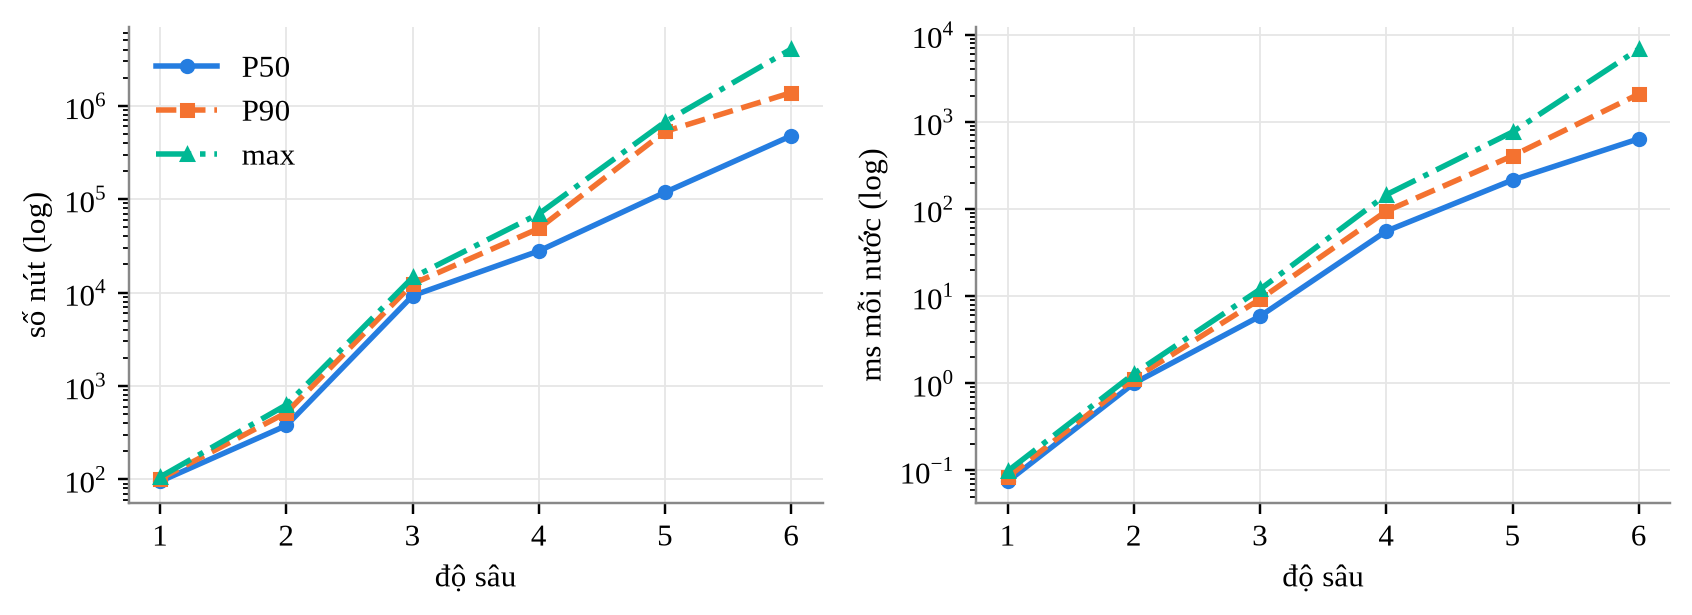
\includegraphics[width=\linewidth]{chuyen-sau/hinh/tk-do-sau.png}
  \caption{Số nút và thời gian mỗi nước của L3 theo độ sâu (thang log).}
  \label{fig:cs-tk-do-sau}
\end{figure}
Tỷ số số nút giữa hai độ sâu liên tiếp dao động theo tính chẵn lẻ: lên độ sâu lẻ nhân khoảng $20$ rồi $6{,}7$ lần,
lên độ sâu chẵn chỉ khoảng $3{,}5$ lần. Đó là dấu hiệu của cây tối thiểu ở định lý~\ref{dl:cs-knuth-moore}: số lá
$b^{\lceil d/2\rceil}+b^{\lfloor d/2\rfloor}-1$ tăng mạnh khi $\lceil d/2\rceil$ tăng. Nước chọn ở các độ sâu nông
trùng với độ sâu 6 chỉ ở $38$--$64\%$ số thế: ngay cả độ sâu 5 cũng chưa ổn định. Độ lệch giữa trung vị và phân vị 95
lớn ở độ sâu 6, nên ngân sách theo độ sâu cho thời gian mỗi nước rất không đều.

\subsection{Python và Cython}
\begin{table}[H]
  \centering
  \small
  \caption{L3: Python thuần so với lõi Cython trên 20 thế}
  \label{tab:cs-tk-backend-ab}
  \begin{tabular}{rrrrrr}
    \toprule
    Độ sâu & Python P50 (ms) & Cython P50 (ms) & Tăng tốc & Cùng số nút & Cùng nước \\
    \midrule
    2 & 24,9 & 1,06 & 25,4 & 20/20 & 20/20 \\
    3 & 300,0 & 6,41 & 38,5 & 20/20 & 20/20 \\
    4 & 1675,4 & 63,97 & 27,9 & 20/20 & 20/20 \\
    \bottomrule
  \end{tabular}
\end{table}

Ở Alpha-Beta, lõi Cython nhanh hơn khoảng $25$--$39$ lần, với số nút và nước chọn trùng khớp trên cả 20 thế ở mọi độ
sâu: đúng yêu cầu thiết kế ``cùng tìm kiếm, khác tốc độ''.
\begin{table}[H]
  \centering
  \footnotesize
  \caption{PUCT 200 mô phỏng: backend và số lá mỗi lô, 20 thế}
  \label{tab:cs-tk-backend-puct}
  \begin{tabular}{lrrrrr}
    \toprule
    Tác tử & Lô & Python P50 (ms) & Cython P50 (ms) & Tăng tốc & Cùng nước với lô 1 \\
    \midrule
    L7 & 1 & 203,1 & 323,9 & 0,67 & 20/20 \\
    L7 & 4 & 128,1 & 163,5 & 0,77 & 19/20 \\
    L7 & 8 & 115,3 & 99,5 & 1,03 & 19/20 \\
    L7 & 16 & 140,3 & 105,2 & 1,34 & 17/20 \\
    L7 & 32 & 151,4 & 113,2 & 1,26 & 15/20 \\
    \midrule
    L8 & 1 & 265,7 & 250,2 & 1,04 & 20/20 \\
    L8 & 4 & 161,4 & 147,0 & 1,14 & 18/20 \\
    L8 & 8 & 118,8 & 101,4 & 1,14 & 15/20 \\
    L8 & 16 & 104,8 & 96,1 & 1,10 & 14/20 \\
    L8 & 32 & 111,6 & 110,5 & 1,01 & 13/20 \\
    \bottomrule
  \end{tabular}
\end{table}

Với PUCT, backend gần như không đổi thời gian (tỷ số dao động quanh 1, một ô thậm chí chậm hơn), vì thời gian bị chi
phối bởi suy luận mạng trên CPU; phần chọn con được Cython hoá quá nhỏ để thấy qua nhiễu đo. Gom lá mới là yếu tố tăng
tốc: từ lô 1 lên lô 8 giảm thời gian khoảng 40 đến 70\%. Đổi lại, lô lớn đổi nước chọn so với tìm kiếm tuần
tự: ở lô 32, chỉ 13--15 trên 20 thế giữ cùng nước. Trên bộ chiến thuật (Bảng~\ref{tab:cs-ct-batch}) sự đổi nước này
không làm giảm tỷ lệ đúng; tác động lên sức chơi chưa đo.

\subsection{MCTS và suy luận mạng}
\begin{table}[H]
  \centering
  \small
  \caption{Thông lượng MCTS (Python) theo kiểu rollout}
  \label{tab:cs-tk-mcts}
  \begin{tabular}{lrrrr}
    \toprule
    Rollout & Mô phỏng & P50 (ms) & Mô phỏng/s & µs/mô phỏng \\
    \midrule
    random & 100 & 21,4 & 4.673 & 214 \\
    random & 400 & 77,9 & 5.132 & 195 \\
    random & 800 & 163,9 & 4.881 & 205 \\
    random & 1.600 & 320,0 & 5.000 & 200 \\
    light & 100 & 82,3 & 1.215 & 823 \\
    light & 400 & 290,5 & 1.377 & 726 \\
    light & 800 & 542,9 & 1.474 & 679 \\
    light & 1.600 & 1055,6 & 1.516 & 660 \\
    \bottomrule
  \end{tabular}
\end{table}

MCTS Python đạt khoảng $5\,000$ mô phỏng mỗi giây với rollout ngẫu nhiên và $1\,200$--$1\,500$ với \texttt{light}. So với
thời gian một rollout ở Bảng~\ref{tab:cs-tk-vi-mo}, rollout chiếm phần lớn mỗi mô phỏng; tối ưu cây không giúp bao
nhiêu nếu rollout vẫn viết bằng Python.
\begin{table}[H]
  \centering
  \small
  \caption{Suy luận mạng trên CPU: ms mỗi lô / số thế mỗi giây}
  \label{tab:cs-tk-thongluong}
  \begin{tabular}{rrrr}
    \toprule
    Lô & 1 luồng & 4 luồng & 8 luồng \\
    \midrule
    1 & 1,97 / 508 & 0,86 / 1.156 & 0,87 / 1.151 \\
    2 & 2,61 / 767 & 1,61 / 1.241 & 1,56 / 1.281 \\
    4 & 4,32 / 925 & 2,13 / 1.876 & 1,91 / 2.093 \\
    8 & 7,53 / 1.062 & 3,09 / 2.586 & 2,40 / 3.339 \\
    16 & 14,61 / 1.095 & 5,04 / 3.178 & 3,41 / 4.687 \\
    32 & 28,30 / 1.131 & 8,97 / 3.567 & 5,43 / 5.892 \\
    64 & 70,30 / 910 & 17,20 / 3.721 & 9,87 / 6.486 \\
    256 & 326,02 / 785 & 139,07 / 1.841 & 90,40 / 2.832 \\
    \bottomrule
  \end{tabular}
\end{table}

\begin{figure}[H]
  \centering
  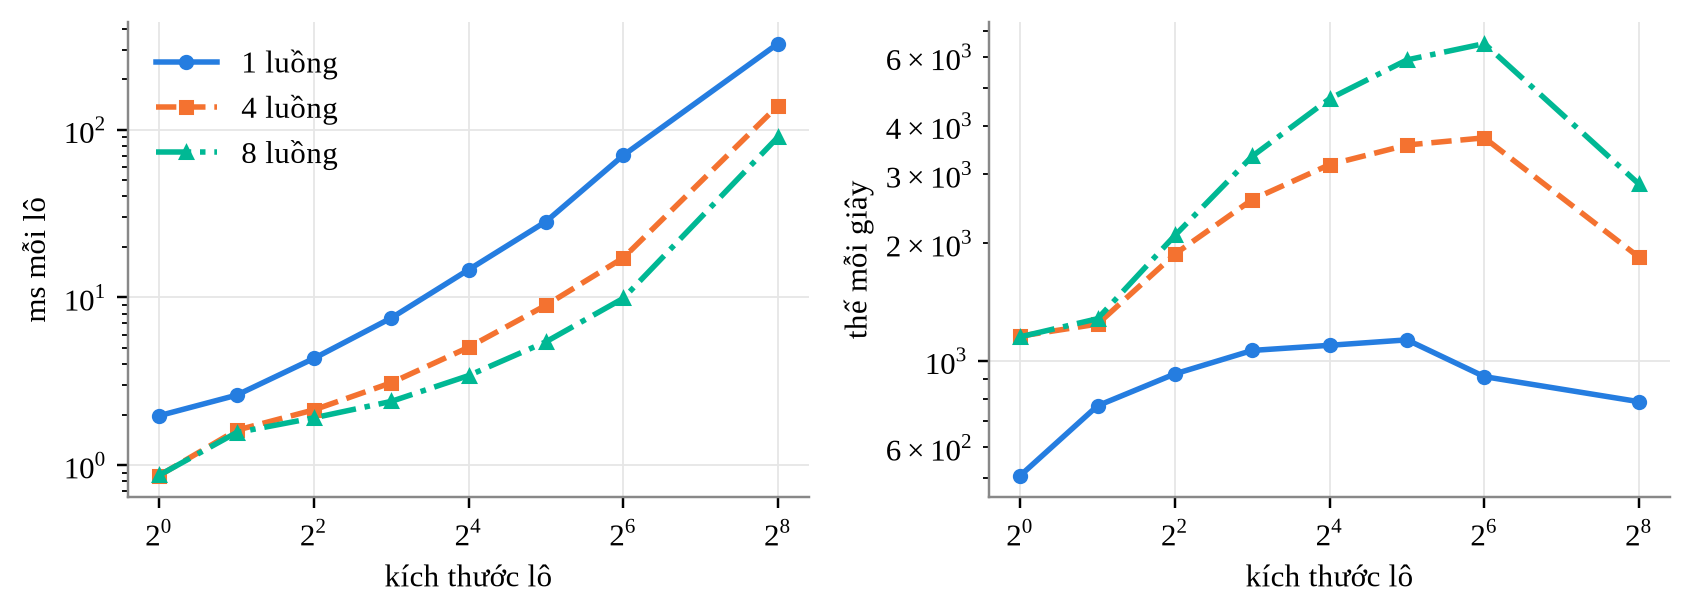
\includegraphics[width=\linewidth]{chuyen-sau/hinh/tk-thong-luong.png}
  \caption{Thời gian mỗi lô và thông lượng suy luận trên CPU theo kích thước lô và số luồng.}
  \label{fig:cs-tk-thong-luong}
\end{figure}
Trên CPU, thông lượng tăng theo lô tới khoảng 32--64 thế rồi giảm ở lô 256, khi dữ liệu trung gian không còn vừa bộ đệm.
Bốn luồng cho gấp đôi một luồng ở lô 1; thêm luồng nữa chỉ có lợi ở lô lớn. Vì giải đấu chạy một tiến trình dùng nhiều
luồng, thời gian mỗi nước của L7, L8 nhạy với tải máy, một lời giải thích khả dĩ (chưa kiểm chứng) cho chênh lệch
thời gian giữa hai lượt RR8 đã nêu ở Mục~\ref{sec:chi-phi-tg}.

\subsection{Lượt thăm thay đổi thế nào khi tăng ngân sách}
\begin{table}[H]
  \centering
  \footnotesize
  \caption{Tìm kiếm tại thế C3-001}
  \label{tab:cs-tk-nhiet-c3-001}
  \begin{tabular}{lrcrrl}
    \toprule
    Cấu hình & Mô phỏng & Chọn & Thăm đáp án (\%) & Q & Biến chính \\
    \midrule
    L4 light & 100 & J7 & 20,0 & 1,00 & J7 K5 \\
    L4 light & 800 & J3 & 60,4 & 1,00 & J3 B10 \\
    L4 light & 6.400 & K2 & 41,0 & 0,27 & K2 D5 J3 \\
    L7 & 50 & I7 & 100,0 & 1,00 & I7 E1 \\
    L7 & 800 & I7 & 100,0 & 1,00 & I7 B11 I8 \\
    L7 & 3.200 & I7 & 100,0 & 1,00 & I7 B11 I8 \\
    L8 & 50 & I3 & 90,0 & 1,00 & I3 D1 \\
    L8 & 800 & I3 & 99,4 & 1,00 & I3 D5 I2 \\
    L8 & 3.200 & I3 & 99,8 & 1,00 & I3 D5 I2 \\
    \bottomrule
  \end{tabular}
\end{table}

\begin{figure}[H]
  \centering
  \begin{subfigure}[t]{.32\linewidth}
    \centering
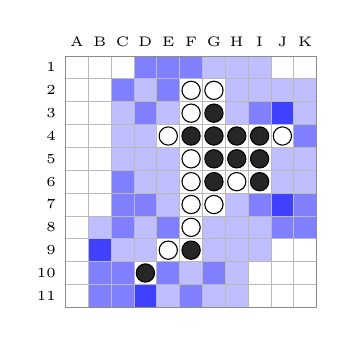
\begin{tikzpicture}[x=0.29cm, y=0.29cm]
\fill[blue!25] (4,-2) rectangle (5,-3);
\fill[blue!75] (3,-10) rectangle (4,-11);
\fill[blue!25] (8,-7) rectangle (9,-8);
\fill[blue!75] (9,-6) rectangle (10,-7);
\fill[blue!50] (2,-7) rectangle (3,-8);
\fill[blue!50] (4,-9) rectangle (5,-10);
\fill[blue!25] (6,-7) rectangle (7,-8);
\fill[blue!75] (1,-8) rectangle (2,-9);
\fill[blue!25] (7,-9) rectangle (8,-10);
\fill[blue!75] (9,-2) rectangle (10,-3);
\fill[blue!25] (1,-7) rectangle (2,-8);
\fill[blue!50] (2,-5) rectangle (3,-6);
\fill[blue!25] (7,-6) rectangle (8,-7);
\fill[blue!25] (9,-5) rectangle (10,-6);
\fill[blue!25] (8,-1) rectangle (9,-2);
\fill[blue!50] (3,-6) rectangle (4,-7);
\fill[blue!50] (3,0) rectangle (4,-1);
\fill[blue!50] (2,-9) rectangle (3,-10);
\fill[blue!50] (1,-9) rectangle (2,-10);
\fill[blue!25] (2,-3) rectangle (3,-4);
\fill[blue!50] (4,-1) rectangle (5,-2);
\fill[blue!50] (8,-6) rectangle (9,-7);
\fill[blue!50] (5,-10) rectangle (6,-11);
\fill[blue!25] (7,0) rectangle (8,-1);
\fill[blue!50] (10,-6) rectangle (11,-7);
\fill[blue!25] (7,-2) rectangle (8,-3);
\fill[blue!50] (8,-2) rectangle (9,-3);
\fill[blue!50] (6,-9) rectangle (7,-10);
\fill[blue!25] (8,-8) rectangle (9,-9);
\fill[blue!25] (2,-4) rectangle (3,-5);
\fill[blue!25] (4,-10) rectangle (5,-11);
\fill[blue!25] (10,-1) rectangle (11,-2);
\fill[blue!50] (3,-2) rectangle (4,-3);
\fill[blue!50] (2,-6) rectangle (3,-7);
\fill[blue!25] (4,-6) rectangle (5,-7);
\fill[blue!25] (6,-10) rectangle (7,-11);
\fill[blue!25] (4,-5) rectangle (5,-6);
\fill[blue!25] (2,-2) rectangle (3,-3);
\fill[blue!25] (10,-4) rectangle (11,-5);
\fill[blue!25] (2,-8) rectangle (3,-9);
\fill[blue!50] (10,-7) rectangle (11,-8);
\fill[blue!25] (7,-8) rectangle (8,-9);
\fill[blue!25] (10,-2) rectangle (11,-3);
\fill[blue!25] (3,-7) rectangle (4,-8);
\fill[blue!25] (6,-8) rectangle (7,-9);
\fill[blue!25] (3,-3) rectangle (4,-4);
\fill[blue!25] (3,-1) rectangle (4,-2);
\fill[blue!50] (10,-3) rectangle (11,-4);
\fill[blue!25] (5,-9) rectangle (6,-10);
\fill[blue!25] (7,-1) rectangle (8,-2);
\fill[blue!25] (9,-1) rectangle (10,-2);
\fill[blue!25] (7,-7) rectangle (8,-8);
\fill[blue!50] (2,-10) rectangle (3,-11);
\fill[blue!50] (5,0) rectangle (6,-1);
\fill[blue!25] (3,-5) rectangle (4,-6);
\fill[blue!25] (4,-4) rectangle (5,-5);
\fill[blue!50] (2,-1) rectangle (3,-2);
\fill[blue!50] (1,-10) rectangle (2,-11);
\fill[blue!25] (7,-10) rectangle (8,-11);
\fill[blue!25] (10,-5) rectangle (11,-6);
\fill[blue!25] (6,0) rectangle (7,-1);
\fill[blue!50] (4,-7) rectangle (5,-8);
\fill[blue!25] (3,-4) rectangle (4,-5);
\fill[blue!25] (8,0) rectangle (9,-1);
\fill[blue!50] (4,0) rectangle (5,-1);
\fill[blue!25] (9,-4) rectangle (10,-5);
\fill[blue!25] (3,-8) rectangle (4,-9);
\fill[blue!50] (9,-7) rectangle (10,-8);
\draw[gray!55, line width=.3pt, step=1] (0,0) grid (11,-11);
\draw[gray!90] (0,0) rectangle (11,-11);
\node[font=\tiny, anchor=south] at (0.5,0) {A};
\node[font=\tiny, anchor=south] at (1.5,0) {B};
\node[font=\tiny, anchor=south] at (2.5,0) {C};
\node[font=\tiny, anchor=south] at (3.5,0) {D};
\node[font=\tiny, anchor=south] at (4.5,0) {E};
\node[font=\tiny, anchor=south] at (5.5,0) {F};
\node[font=\tiny, anchor=south] at (6.5,0) {G};
\node[font=\tiny, anchor=south] at (7.5,0) {H};
\node[font=\tiny, anchor=south] at (8.5,0) {I};
\node[font=\tiny, anchor=south] at (9.5,0) {J};
\node[font=\tiny, anchor=south] at (10.5,0) {K};
\node[font=\tiny, anchor=east] at (0,-0.5) {1};
\node[font=\tiny, anchor=east] at (0,-1.5) {2};
\node[font=\tiny, anchor=east] at (0,-2.5) {3};
\node[font=\tiny, anchor=east] at (0,-3.5) {4};
\node[font=\tiny, anchor=east] at (0,-4.5) {5};
\node[font=\tiny, anchor=east] at (0,-5.5) {6};
\node[font=\tiny, anchor=east] at (0,-6.5) {7};
\node[font=\tiny, anchor=east] at (0,-7.5) {8};
\node[font=\tiny, anchor=east] at (0,-8.5) {9};
\node[font=\tiny, anchor=east] at (0,-9.5) {10};
\node[font=\tiny, anchor=east] at (0,-10.5) {11};
\draw[fill=white, line width=.4pt] (5.5,-1.5) circle (.40);
\draw[fill=white, line width=.4pt] (6.5,-1.5) circle (.40);
\draw[fill=white, line width=.4pt] (5.5,-2.5) circle (.40);
\draw[fill=black!85, line width=.4pt] (6.5,-2.5) circle (.40);
\draw[fill=white, line width=.4pt] (4.5,-3.5) circle (.40);
\draw[fill=black!85, line width=.4pt] (5.5,-3.5) circle (.40);
\draw[fill=black!85, line width=.4pt] (6.5,-3.5) circle (.40);
\draw[fill=black!85, line width=.4pt] (7.5,-3.5) circle (.40);
\draw[fill=black!85, line width=.4pt] (8.5,-3.5) circle (.40);
\draw[fill=white, line width=.4pt] (9.5,-3.5) circle (.40);
\draw[fill=white, line width=.4pt] (5.5,-4.5) circle (.40);
\draw[fill=black!85, line width=.4pt] (6.5,-4.5) circle (.40);
\draw[fill=black!85, line width=.4pt] (7.5,-4.5) circle (.40);
\draw[fill=black!85, line width=.4pt] (8.5,-4.5) circle (.40);
\draw[fill=white, line width=.4pt] (5.5,-5.5) circle (.40);
\draw[fill=black!85, line width=.4pt] (6.5,-5.5) circle (.40);
\draw[fill=white, line width=.4pt] (7.5,-5.5) circle (.40);
\draw[fill=black!85, line width=.4pt] (8.5,-5.5) circle (.40);
\draw[fill=white, line width=.4pt] (5.5,-6.5) circle (.40);
\draw[fill=white, line width=.4pt] (6.5,-6.5) circle (.40);
\draw[fill=white, line width=.4pt] (5.5,-7.5) circle (.40);
\draw[fill=white, line width=.4pt] (4.5,-8.5) circle (.40);
\draw[fill=black!85, line width=.4pt] (5.5,-8.5) circle (.40);
\draw[fill=black!85, line width=.4pt] (3.5,-9.5) circle (.40);
\end{tikzpicture}
    \caption{\footnotesize L4 light, 100: J7}
  \end{subfigure}\hfill
  \begin{subfigure}[t]{.32\linewidth}
    \centering
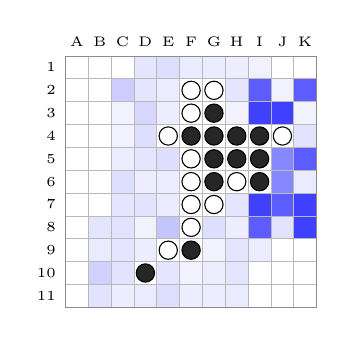
\begin{tikzpicture}[x=0.29cm, y=0.29cm]
\fill[blue!7] (4,-2) rectangle (5,-3);
\fill[blue!8] (3,-10) rectangle (4,-11);
\fill[blue!64] (8,-7) rectangle (9,-8);
\fill[blue!64] (9,-6) rectangle (10,-7);
\fill[blue!11] (2,-7) rectangle (3,-8);
\fill[blue!10] (4,-9) rectangle (5,-10);
\fill[blue!13] (6,-7) rectangle (7,-8);
\fill[blue!8] (1,-8) rectangle (2,-9);
\fill[blue!10] (7,-9) rectangle (8,-10);
\fill[blue!75] (9,-2) rectangle (10,-3);
\fill[blue!10] (1,-7) rectangle (2,-8);
\fill[blue!13] (2,-5) rectangle (3,-6);
\fill[blue!10] (7,-6) rectangle (8,-7);
\fill[blue!47] (9,-5) rectangle (10,-6);
\fill[blue!64] (8,-1) rectangle (9,-2);
\fill[blue!11] (3,-6) rectangle (4,-7);
\fill[blue!10] (3,0) rectangle (4,-1);
\fill[blue!11] (2,-9) rectangle (3,-10);
\fill[blue!18] (1,-9) rectangle (2,-10);
\fill[blue!5] (2,-3) rectangle (3,-4);
\fill[blue!7] (4,-1) rectangle (5,-2);
\fill[blue!75] (8,-6) rectangle (9,-7);
\fill[blue!7] (5,-10) rectangle (6,-11);
\fill[blue!7] (7,0) rectangle (8,-1);
\fill[blue!75] (10,-6) rectangle (11,-7);
\fill[blue!5] (7,-2) rectangle (8,-3);
\fill[blue!75] (8,-2) rectangle (9,-3);
\fill[blue!7] (6,-9) rectangle (7,-10);
\fill[blue!7] (8,-8) rectangle (9,-9);
\fill[blue!7] (2,-4) rectangle (3,-5);
\fill[blue!13] (4,-10) rectangle (5,-11);
\fill[blue!64] (10,-1) rectangle (11,-2);
\fill[blue!16] (3,-2) rectangle (4,-3);
\fill[blue!10] (2,-6) rectangle (3,-7);
\fill[blue!8] (4,-6) rectangle (5,-7);
\fill[blue!7] (6,-10) rectangle (7,-11);
\fill[blue!7] (4,-5) rectangle (5,-6);
\fill[blue!5] (2,-2) rectangle (3,-3);
\fill[blue!64] (10,-4) rectangle (11,-5);
\fill[blue!10] (2,-8) rectangle (3,-9);
\fill[blue!75] (10,-7) rectangle (11,-8);
\fill[blue!10] (7,-8) rectangle (8,-9);
\fill[blue!5] (10,-2) rectangle (11,-3);
\fill[blue!5] (3,-7) rectangle (4,-8);
\fill[blue!5] (6,-8) rectangle (7,-9);
\fill[blue!13] (3,-3) rectangle (4,-4);
\fill[blue!10] (3,-1) rectangle (4,-2);
\fill[blue!11] (10,-3) rectangle (11,-4);
\fill[blue!5] (5,-9) rectangle (6,-10);
\fill[blue!10] (7,-1) rectangle (8,-2);
\fill[blue!5] (9,-1) rectangle (10,-2);
\fill[blue!7] (7,-7) rectangle (8,-8);
\fill[blue!7] (2,-10) rectangle (3,-11);
\fill[blue!8] (5,0) rectangle (6,-1);
\fill[blue!7] (3,-5) rectangle (4,-6);
\fill[blue!13] (4,-4) rectangle (5,-5);
\fill[blue!20] (2,-1) rectangle (3,-2);
\fill[blue!11] (1,-10) rectangle (2,-11);
\fill[blue!8] (7,-10) rectangle (8,-11);
\fill[blue!8] (10,-5) rectangle (11,-6);
\fill[blue!8] (6,0) rectangle (7,-1);
\fill[blue!23] (4,-7) rectangle (5,-8);
\fill[blue!10] (3,-4) rectangle (4,-5);
\fill[blue!5] (8,0) rectangle (9,-1);
\fill[blue!13] (4,0) rectangle (5,-1);
\fill[blue!47] (9,-4) rectangle (10,-5);
\fill[blue!7] (3,-8) rectangle (4,-9);
\fill[blue!11] (9,-7) rectangle (10,-8);
\draw[gray!55, line width=.3pt, step=1] (0,0) grid (11,-11);
\draw[gray!90] (0,0) rectangle (11,-11);
\node[font=\tiny, anchor=south] at (0.5,0) {A};
\node[font=\tiny, anchor=south] at (1.5,0) {B};
\node[font=\tiny, anchor=south] at (2.5,0) {C};
\node[font=\tiny, anchor=south] at (3.5,0) {D};
\node[font=\tiny, anchor=south] at (4.5,0) {E};
\node[font=\tiny, anchor=south] at (5.5,0) {F};
\node[font=\tiny, anchor=south] at (6.5,0) {G};
\node[font=\tiny, anchor=south] at (7.5,0) {H};
\node[font=\tiny, anchor=south] at (8.5,0) {I};
\node[font=\tiny, anchor=south] at (9.5,0) {J};
\node[font=\tiny, anchor=south] at (10.5,0) {K};
\node[font=\tiny, anchor=east] at (0,-0.5) {1};
\node[font=\tiny, anchor=east] at (0,-1.5) {2};
\node[font=\tiny, anchor=east] at (0,-2.5) {3};
\node[font=\tiny, anchor=east] at (0,-3.5) {4};
\node[font=\tiny, anchor=east] at (0,-4.5) {5};
\node[font=\tiny, anchor=east] at (0,-5.5) {6};
\node[font=\tiny, anchor=east] at (0,-6.5) {7};
\node[font=\tiny, anchor=east] at (0,-7.5) {8};
\node[font=\tiny, anchor=east] at (0,-8.5) {9};
\node[font=\tiny, anchor=east] at (0,-9.5) {10};
\node[font=\tiny, anchor=east] at (0,-10.5) {11};
\draw[fill=white, line width=.4pt] (5.5,-1.5) circle (.40);
\draw[fill=white, line width=.4pt] (6.5,-1.5) circle (.40);
\draw[fill=white, line width=.4pt] (5.5,-2.5) circle (.40);
\draw[fill=black!85, line width=.4pt] (6.5,-2.5) circle (.40);
\draw[fill=white, line width=.4pt] (4.5,-3.5) circle (.40);
\draw[fill=black!85, line width=.4pt] (5.5,-3.5) circle (.40);
\draw[fill=black!85, line width=.4pt] (6.5,-3.5) circle (.40);
\draw[fill=black!85, line width=.4pt] (7.5,-3.5) circle (.40);
\draw[fill=black!85, line width=.4pt] (8.5,-3.5) circle (.40);
\draw[fill=white, line width=.4pt] (9.5,-3.5) circle (.40);
\draw[fill=white, line width=.4pt] (5.5,-4.5) circle (.40);
\draw[fill=black!85, line width=.4pt] (6.5,-4.5) circle (.40);
\draw[fill=black!85, line width=.4pt] (7.5,-4.5) circle (.40);
\draw[fill=black!85, line width=.4pt] (8.5,-4.5) circle (.40);
\draw[fill=white, line width=.4pt] (5.5,-5.5) circle (.40);
\draw[fill=black!85, line width=.4pt] (6.5,-5.5) circle (.40);
\draw[fill=white, line width=.4pt] (7.5,-5.5) circle (.40);
\draw[fill=black!85, line width=.4pt] (8.5,-5.5) circle (.40);
\draw[fill=white, line width=.4pt] (5.5,-6.5) circle (.40);
\draw[fill=white, line width=.4pt] (6.5,-6.5) circle (.40);
\draw[fill=white, line width=.4pt] (5.5,-7.5) circle (.40);
\draw[fill=white, line width=.4pt] (4.5,-8.5) circle (.40);
\draw[fill=black!85, line width=.4pt] (5.5,-8.5) circle (.40);
\draw[fill=black!85, line width=.4pt] (3.5,-9.5) circle (.40);
\end{tikzpicture}
    \caption{\footnotesize L4 light, 800: J3}
  \end{subfigure}\hfill
  \begin{subfigure}[t]{.32\linewidth}
    \centering
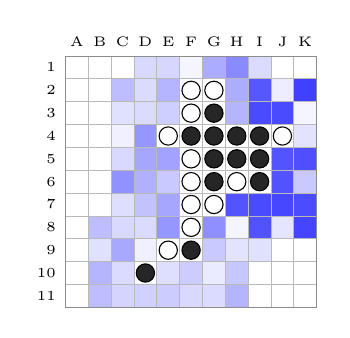
\begin{tikzpicture}[x=0.29cm, y=0.29cm]
\fill[blue!19] (4,-2) rectangle (5,-3);
\fill[blue!18] (3,-10) rectangle (4,-11);
\fill[blue!68] (8,-7) rectangle (9,-8);
\fill[blue!72] (9,-6) rectangle (10,-7);
\fill[blue!15] (2,-7) rectangle (3,-8);
\fill[blue!13] (4,-9) rectangle (5,-10);
\fill[blue!44] (6,-7) rectangle (7,-8);
\fill[blue!12] (1,-8) rectangle (2,-9);
\fill[blue!22] (7,-9) rectangle (8,-10);
\fill[blue!71] (9,-2) rectangle (10,-3);
\fill[blue!26] (1,-7) rectangle (2,-8);
\fill[blue!43] (2,-5) rectangle (3,-6);
\fill[blue!67] (7,-6) rectangle (8,-7);
\fill[blue!68] (9,-5) rectangle (10,-6);
\fill[blue!66] (8,-1) rectangle (9,-2);
\fill[blue!24] (3,-6) rectangle (4,-7);
\fill[blue!15] (3,0) rectangle (4,-1);
\fill[blue!14] (2,-9) rectangle (3,-10);
\fill[blue!29] (1,-9) rectangle (2,-10);
\fill[blue!6] (2,-3) rectangle (3,-4);
\fill[blue!29] (4,-1) rectangle (5,-2);
\fill[blue!71] (8,-6) rectangle (9,-7);
\fill[blue!15] (5,-10) rectangle (6,-11);
\fill[blue!46] (7,0) rectangle (8,-1);
\fill[blue!70] (10,-6) rectangle (11,-7);
\fill[blue!29] (7,-2) rectangle (8,-3);
\fill[blue!71] (8,-2) rectangle (9,-3);
\fill[blue!8] (6,-9) rectangle (7,-10);
\fill[blue!12] (8,-8) rectangle (9,-9);
\fill[blue!15] (2,-4) rectangle (3,-5);
\fill[blue!20] (4,-10) rectangle (5,-11);
\fill[blue!75] (10,-1) rectangle (11,-2);
\fill[blue!14] (3,-2) rectangle (4,-3);
\fill[blue!13] (2,-6) rectangle (3,-7);
\fill[blue!35] (4,-6) rectangle (5,-7);
\fill[blue!14] (6,-10) rectangle (7,-11);
\fill[blue!21] (4,-5) rectangle (5,-6);
\fill[blue!12] (2,-2) rectangle (3,-3);
\fill[blue!69] (10,-4) rectangle (11,-5);
\fill[blue!34] (2,-8) rectangle (3,-9);
\fill[blue!73] (10,-7) rectangle (11,-8);
\fill[blue!11] (7,-8) rectangle (8,-9);
\fill[blue!4] (10,-2) rectangle (11,-3);
\fill[blue!14] (3,-7) rectangle (4,-8);
\fill[blue!21] (6,-8) rectangle (7,-9);
\fill[blue!41] (3,-3) rectangle (4,-4);
\fill[blue!14] (3,-1) rectangle (4,-2);
\fill[blue!11] (10,-3) rectangle (11,-4);
\fill[blue!20] (5,-9) rectangle (6,-10);
\fill[blue!32] (7,-1) rectangle (8,-2);
\fill[blue!7] (9,-1) rectangle (10,-2);
\fill[blue!4] (7,-7) rectangle (8,-8);
\fill[blue!17] (2,-10) rectangle (3,-11);
\fill[blue!4] (5,0) rectangle (6,-1);
\fill[blue!31] (3,-5) rectangle (4,-6);
\fill[blue!36] (4,-4) rectangle (5,-5);
\fill[blue!26] (2,-1) rectangle (3,-2);
\fill[blue!26] (1,-10) rectangle (2,-11);
\fill[blue!29] (7,-10) rectangle (8,-11);
\fill[blue!21] (10,-5) rectangle (11,-6);
\fill[blue!33] (6,0) rectangle (7,-1);
\fill[blue!41] (4,-7) rectangle (5,-8);
\fill[blue!35] (3,-4) rectangle (4,-5);
\fill[blue!14] (8,0) rectangle (9,-1);
\fill[blue!16] (4,0) rectangle (5,-1);
\fill[blue!67] (9,-4) rectangle (10,-5);
\fill[blue!6] (3,-8) rectangle (4,-9);
\fill[blue!10] (9,-7) rectangle (10,-8);
\draw[gray!55, line width=.3pt, step=1] (0,0) grid (11,-11);
\draw[gray!90] (0,0) rectangle (11,-11);
\node[font=\tiny, anchor=south] at (0.5,0) {A};
\node[font=\tiny, anchor=south] at (1.5,0) {B};
\node[font=\tiny, anchor=south] at (2.5,0) {C};
\node[font=\tiny, anchor=south] at (3.5,0) {D};
\node[font=\tiny, anchor=south] at (4.5,0) {E};
\node[font=\tiny, anchor=south] at (5.5,0) {F};
\node[font=\tiny, anchor=south] at (6.5,0) {G};
\node[font=\tiny, anchor=south] at (7.5,0) {H};
\node[font=\tiny, anchor=south] at (8.5,0) {I};
\node[font=\tiny, anchor=south] at (9.5,0) {J};
\node[font=\tiny, anchor=south] at (10.5,0) {K};
\node[font=\tiny, anchor=east] at (0,-0.5) {1};
\node[font=\tiny, anchor=east] at (0,-1.5) {2};
\node[font=\tiny, anchor=east] at (0,-2.5) {3};
\node[font=\tiny, anchor=east] at (0,-3.5) {4};
\node[font=\tiny, anchor=east] at (0,-4.5) {5};
\node[font=\tiny, anchor=east] at (0,-5.5) {6};
\node[font=\tiny, anchor=east] at (0,-6.5) {7};
\node[font=\tiny, anchor=east] at (0,-7.5) {8};
\node[font=\tiny, anchor=east] at (0,-8.5) {9};
\node[font=\tiny, anchor=east] at (0,-9.5) {10};
\node[font=\tiny, anchor=east] at (0,-10.5) {11};
\draw[fill=white, line width=.4pt] (5.5,-1.5) circle (.40);
\draw[fill=white, line width=.4pt] (6.5,-1.5) circle (.40);
\draw[fill=white, line width=.4pt] (5.5,-2.5) circle (.40);
\draw[fill=black!85, line width=.4pt] (6.5,-2.5) circle (.40);
\draw[fill=white, line width=.4pt] (4.5,-3.5) circle (.40);
\draw[fill=black!85, line width=.4pt] (5.5,-3.5) circle (.40);
\draw[fill=black!85, line width=.4pt] (6.5,-3.5) circle (.40);
\draw[fill=black!85, line width=.4pt] (7.5,-3.5) circle (.40);
\draw[fill=black!85, line width=.4pt] (8.5,-3.5) circle (.40);
\draw[fill=white, line width=.4pt] (9.5,-3.5) circle (.40);
\draw[fill=white, line width=.4pt] (5.5,-4.5) circle (.40);
\draw[fill=black!85, line width=.4pt] (6.5,-4.5) circle (.40);
\draw[fill=black!85, line width=.4pt] (7.5,-4.5) circle (.40);
\draw[fill=black!85, line width=.4pt] (8.5,-4.5) circle (.40);
\draw[fill=white, line width=.4pt] (5.5,-5.5) circle (.40);
\draw[fill=black!85, line width=.4pt] (6.5,-5.5) circle (.40);
\draw[fill=white, line width=.4pt] (7.5,-5.5) circle (.40);
\draw[fill=black!85, line width=.4pt] (8.5,-5.5) circle (.40);
\draw[fill=white, line width=.4pt] (5.5,-6.5) circle (.40);
\draw[fill=white, line width=.4pt] (6.5,-6.5) circle (.40);
\draw[fill=white, line width=.4pt] (5.5,-7.5) circle (.40);
\draw[fill=white, line width=.4pt] (4.5,-8.5) circle (.40);
\draw[fill=black!85, line width=.4pt] (5.5,-8.5) circle (.40);
\draw[fill=black!85, line width=.4pt] (3.5,-9.5) circle (.40);
\end{tikzpicture}
    \caption{\footnotesize L4 light, 6.400: K2}
  \end{subfigure}\par\medskip
  \begin{subfigure}[t]{.32\linewidth}
    \centering
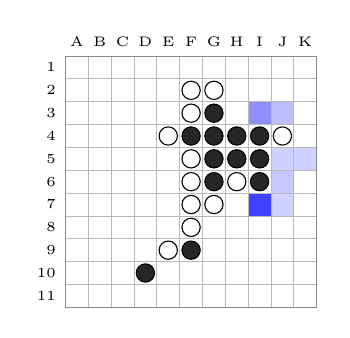
\begin{tikzpicture}[x=0.29cm, y=0.29cm]
\fill[blue!44] (8,-2) rectangle (9,-3);
\fill[blue!26] (9,-2) rectangle (10,-3);
\fill[blue!18] (9,-4) rectangle (10,-5);
\fill[blue!18] (10,-4) rectangle (11,-5);
\fill[blue!22] (9,-5) rectangle (10,-6);
\fill[blue!75] (8,-6) rectangle (9,-7);
\fill[blue!18] (9,-6) rectangle (10,-7);
\draw[gray!55, line width=.3pt, step=1] (0,0) grid (11,-11);
\draw[gray!90] (0,0) rectangle (11,-11);
\node[font=\tiny, anchor=south] at (0.5,0) {A};
\node[font=\tiny, anchor=south] at (1.5,0) {B};
\node[font=\tiny, anchor=south] at (2.5,0) {C};
\node[font=\tiny, anchor=south] at (3.5,0) {D};
\node[font=\tiny, anchor=south] at (4.5,0) {E};
\node[font=\tiny, anchor=south] at (5.5,0) {F};
\node[font=\tiny, anchor=south] at (6.5,0) {G};
\node[font=\tiny, anchor=south] at (7.5,0) {H};
\node[font=\tiny, anchor=south] at (8.5,0) {I};
\node[font=\tiny, anchor=south] at (9.5,0) {J};
\node[font=\tiny, anchor=south] at (10.5,0) {K};
\node[font=\tiny, anchor=east] at (0,-0.5) {1};
\node[font=\tiny, anchor=east] at (0,-1.5) {2};
\node[font=\tiny, anchor=east] at (0,-2.5) {3};
\node[font=\tiny, anchor=east] at (0,-3.5) {4};
\node[font=\tiny, anchor=east] at (0,-4.5) {5};
\node[font=\tiny, anchor=east] at (0,-5.5) {6};
\node[font=\tiny, anchor=east] at (0,-6.5) {7};
\node[font=\tiny, anchor=east] at (0,-7.5) {8};
\node[font=\tiny, anchor=east] at (0,-8.5) {9};
\node[font=\tiny, anchor=east] at (0,-9.5) {10};
\node[font=\tiny, anchor=east] at (0,-10.5) {11};
\draw[fill=white, line width=.4pt] (5.5,-1.5) circle (.40);
\draw[fill=white, line width=.4pt] (6.5,-1.5) circle (.40);
\draw[fill=white, line width=.4pt] (5.5,-2.5) circle (.40);
\draw[fill=black!85, line width=.4pt] (6.5,-2.5) circle (.40);
\draw[fill=white, line width=.4pt] (4.5,-3.5) circle (.40);
\draw[fill=black!85, line width=.4pt] (5.5,-3.5) circle (.40);
\draw[fill=black!85, line width=.4pt] (6.5,-3.5) circle (.40);
\draw[fill=black!85, line width=.4pt] (7.5,-3.5) circle (.40);
\draw[fill=black!85, line width=.4pt] (8.5,-3.5) circle (.40);
\draw[fill=white, line width=.4pt] (9.5,-3.5) circle (.40);
\draw[fill=white, line width=.4pt] (5.5,-4.5) circle (.40);
\draw[fill=black!85, line width=.4pt] (6.5,-4.5) circle (.40);
\draw[fill=black!85, line width=.4pt] (7.5,-4.5) circle (.40);
\draw[fill=black!85, line width=.4pt] (8.5,-4.5) circle (.40);
\draw[fill=white, line width=.4pt] (5.5,-5.5) circle (.40);
\draw[fill=black!85, line width=.4pt] (6.5,-5.5) circle (.40);
\draw[fill=white, line width=.4pt] (7.5,-5.5) circle (.40);
\draw[fill=black!85, line width=.4pt] (8.5,-5.5) circle (.40);
\draw[fill=white, line width=.4pt] (5.5,-6.5) circle (.40);
\draw[fill=white, line width=.4pt] (6.5,-6.5) circle (.40);
\draw[fill=white, line width=.4pt] (5.5,-7.5) circle (.40);
\draw[fill=white, line width=.4pt] (4.5,-8.5) circle (.40);
\draw[fill=black!85, line width=.4pt] (5.5,-8.5) circle (.40);
\draw[fill=black!85, line width=.4pt] (3.5,-9.5) circle (.40);
\end{tikzpicture}
    \caption{\footnotesize L7, 50: I7}
  \end{subfigure}\hfill
  \begin{subfigure}[t]{.32\linewidth}
    \centering
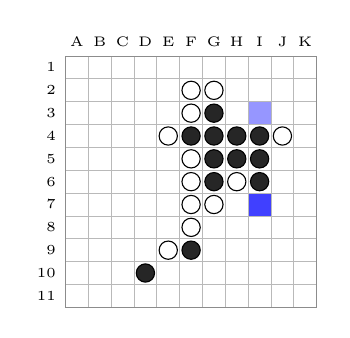
\begin{tikzpicture}[x=0.29cm, y=0.29cm]
\fill[blue!41] (8,-2) rectangle (9,-3);
\fill[blue!75] (8,-6) rectangle (9,-7);
\draw[gray!55, line width=.3pt, step=1] (0,0) grid (11,-11);
\draw[gray!90] (0,0) rectangle (11,-11);
\node[font=\tiny, anchor=south] at (0.5,0) {A};
\node[font=\tiny, anchor=south] at (1.5,0) {B};
\node[font=\tiny, anchor=south] at (2.5,0) {C};
\node[font=\tiny, anchor=south] at (3.5,0) {D};
\node[font=\tiny, anchor=south] at (4.5,0) {E};
\node[font=\tiny, anchor=south] at (5.5,0) {F};
\node[font=\tiny, anchor=south] at (6.5,0) {G};
\node[font=\tiny, anchor=south] at (7.5,0) {H};
\node[font=\tiny, anchor=south] at (8.5,0) {I};
\node[font=\tiny, anchor=south] at (9.5,0) {J};
\node[font=\tiny, anchor=south] at (10.5,0) {K};
\node[font=\tiny, anchor=east] at (0,-0.5) {1};
\node[font=\tiny, anchor=east] at (0,-1.5) {2};
\node[font=\tiny, anchor=east] at (0,-2.5) {3};
\node[font=\tiny, anchor=east] at (0,-3.5) {4};
\node[font=\tiny, anchor=east] at (0,-4.5) {5};
\node[font=\tiny, anchor=east] at (0,-5.5) {6};
\node[font=\tiny, anchor=east] at (0,-6.5) {7};
\node[font=\tiny, anchor=east] at (0,-7.5) {8};
\node[font=\tiny, anchor=east] at (0,-8.5) {9};
\node[font=\tiny, anchor=east] at (0,-9.5) {10};
\node[font=\tiny, anchor=east] at (0,-10.5) {11};
\draw[fill=white, line width=.4pt] (5.5,-1.5) circle (.40);
\draw[fill=white, line width=.4pt] (6.5,-1.5) circle (.40);
\draw[fill=white, line width=.4pt] (5.5,-2.5) circle (.40);
\draw[fill=black!85, line width=.4pt] (6.5,-2.5) circle (.40);
\draw[fill=white, line width=.4pt] (4.5,-3.5) circle (.40);
\draw[fill=black!85, line width=.4pt] (5.5,-3.5) circle (.40);
\draw[fill=black!85, line width=.4pt] (6.5,-3.5) circle (.40);
\draw[fill=black!85, line width=.4pt] (7.5,-3.5) circle (.40);
\draw[fill=black!85, line width=.4pt] (8.5,-3.5) circle (.40);
\draw[fill=white, line width=.4pt] (9.5,-3.5) circle (.40);
\draw[fill=white, line width=.4pt] (5.5,-4.5) circle (.40);
\draw[fill=black!85, line width=.4pt] (6.5,-4.5) circle (.40);
\draw[fill=black!85, line width=.4pt] (7.5,-4.5) circle (.40);
\draw[fill=black!85, line width=.4pt] (8.5,-4.5) circle (.40);
\draw[fill=white, line width=.4pt] (5.5,-5.5) circle (.40);
\draw[fill=black!85, line width=.4pt] (6.5,-5.5) circle (.40);
\draw[fill=white, line width=.4pt] (7.5,-5.5) circle (.40);
\draw[fill=black!85, line width=.4pt] (8.5,-5.5) circle (.40);
\draw[fill=white, line width=.4pt] (5.5,-6.5) circle (.40);
\draw[fill=white, line width=.4pt] (6.5,-6.5) circle (.40);
\draw[fill=white, line width=.4pt] (5.5,-7.5) circle (.40);
\draw[fill=white, line width=.4pt] (4.5,-8.5) circle (.40);
\draw[fill=black!85, line width=.4pt] (5.5,-8.5) circle (.40);
\draw[fill=black!85, line width=.4pt] (3.5,-9.5) circle (.40);
\end{tikzpicture}
    \caption{\footnotesize L7, 800: I7}
  \end{subfigure}\hfill
  \begin{subfigure}[t]{.32\linewidth}
    \centering
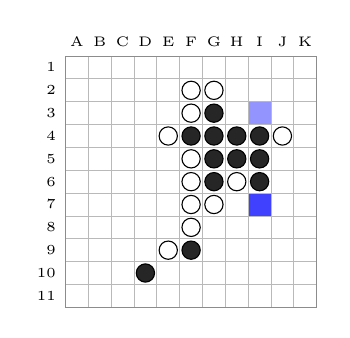
\begin{tikzpicture}[x=0.29cm, y=0.29cm]
\fill[blue!42] (8,-2) rectangle (9,-3);
\fill[blue!75] (8,-6) rectangle (9,-7);
\draw[gray!55, line width=.3pt, step=1] (0,0) grid (11,-11);
\draw[gray!90] (0,0) rectangle (11,-11);
\node[font=\tiny, anchor=south] at (0.5,0) {A};
\node[font=\tiny, anchor=south] at (1.5,0) {B};
\node[font=\tiny, anchor=south] at (2.5,0) {C};
\node[font=\tiny, anchor=south] at (3.5,0) {D};
\node[font=\tiny, anchor=south] at (4.5,0) {E};
\node[font=\tiny, anchor=south] at (5.5,0) {F};
\node[font=\tiny, anchor=south] at (6.5,0) {G};
\node[font=\tiny, anchor=south] at (7.5,0) {H};
\node[font=\tiny, anchor=south] at (8.5,0) {I};
\node[font=\tiny, anchor=south] at (9.5,0) {J};
\node[font=\tiny, anchor=south] at (10.5,0) {K};
\node[font=\tiny, anchor=east] at (0,-0.5) {1};
\node[font=\tiny, anchor=east] at (0,-1.5) {2};
\node[font=\tiny, anchor=east] at (0,-2.5) {3};
\node[font=\tiny, anchor=east] at (0,-3.5) {4};
\node[font=\tiny, anchor=east] at (0,-4.5) {5};
\node[font=\tiny, anchor=east] at (0,-5.5) {6};
\node[font=\tiny, anchor=east] at (0,-6.5) {7};
\node[font=\tiny, anchor=east] at (0,-7.5) {8};
\node[font=\tiny, anchor=east] at (0,-8.5) {9};
\node[font=\tiny, anchor=east] at (0,-9.5) {10};
\node[font=\tiny, anchor=east] at (0,-10.5) {11};
\draw[fill=white, line width=.4pt] (5.5,-1.5) circle (.40);
\draw[fill=white, line width=.4pt] (6.5,-1.5) circle (.40);
\draw[fill=white, line width=.4pt] (5.5,-2.5) circle (.40);
\draw[fill=black!85, line width=.4pt] (6.5,-2.5) circle (.40);
\draw[fill=white, line width=.4pt] (4.5,-3.5) circle (.40);
\draw[fill=black!85, line width=.4pt] (5.5,-3.5) circle (.40);
\draw[fill=black!85, line width=.4pt] (6.5,-3.5) circle (.40);
\draw[fill=black!85, line width=.4pt] (7.5,-3.5) circle (.40);
\draw[fill=black!85, line width=.4pt] (8.5,-3.5) circle (.40);
\draw[fill=white, line width=.4pt] (9.5,-3.5) circle (.40);
\draw[fill=white, line width=.4pt] (5.5,-4.5) circle (.40);
\draw[fill=black!85, line width=.4pt] (6.5,-4.5) circle (.40);
\draw[fill=black!85, line width=.4pt] (7.5,-4.5) circle (.40);
\draw[fill=black!85, line width=.4pt] (8.5,-4.5) circle (.40);
\draw[fill=white, line width=.4pt] (5.5,-5.5) circle (.40);
\draw[fill=black!85, line width=.4pt] (6.5,-5.5) circle (.40);
\draw[fill=white, line width=.4pt] (7.5,-5.5) circle (.40);
\draw[fill=black!85, line width=.4pt] (8.5,-5.5) circle (.40);
\draw[fill=white, line width=.4pt] (5.5,-6.5) circle (.40);
\draw[fill=white, line width=.4pt] (6.5,-6.5) circle (.40);
\draw[fill=white, line width=.4pt] (5.5,-7.5) circle (.40);
\draw[fill=white, line width=.4pt] (4.5,-8.5) circle (.40);
\draw[fill=black!85, line width=.4pt] (5.5,-8.5) circle (.40);
\draw[fill=black!85, line width=.4pt] (3.5,-9.5) circle (.40);
\end{tikzpicture}
    \caption{\footnotesize L7, 3.200: I7}
  \end{subfigure}\par\medskip
  \begin{subfigure}[t]{.32\linewidth}
    \centering
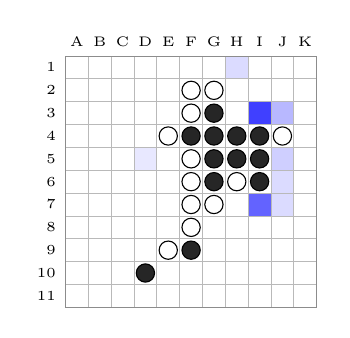
\begin{tikzpicture}[x=0.29cm, y=0.29cm]
\fill[blue!14] (7,0) rectangle (8,-1);
\fill[blue!75] (8,-2) rectangle (9,-3);
\fill[blue!28] (9,-2) rectangle (10,-3);
\fill[blue!9] (3,-4) rectangle (4,-5);
\fill[blue!19] (9,-4) rectangle (10,-5);
\fill[blue!14] (9,-5) rectangle (10,-6);
\fill[blue!61] (8,-6) rectangle (9,-7);
\fill[blue!14] (9,-6) rectangle (10,-7);
\draw[gray!55, line width=.3pt, step=1] (0,0) grid (11,-11);
\draw[gray!90] (0,0) rectangle (11,-11);
\node[font=\tiny, anchor=south] at (0.5,0) {A};
\node[font=\tiny, anchor=south] at (1.5,0) {B};
\node[font=\tiny, anchor=south] at (2.5,0) {C};
\node[font=\tiny, anchor=south] at (3.5,0) {D};
\node[font=\tiny, anchor=south] at (4.5,0) {E};
\node[font=\tiny, anchor=south] at (5.5,0) {F};
\node[font=\tiny, anchor=south] at (6.5,0) {G};
\node[font=\tiny, anchor=south] at (7.5,0) {H};
\node[font=\tiny, anchor=south] at (8.5,0) {I};
\node[font=\tiny, anchor=south] at (9.5,0) {J};
\node[font=\tiny, anchor=south] at (10.5,0) {K};
\node[font=\tiny, anchor=east] at (0,-0.5) {1};
\node[font=\tiny, anchor=east] at (0,-1.5) {2};
\node[font=\tiny, anchor=east] at (0,-2.5) {3};
\node[font=\tiny, anchor=east] at (0,-3.5) {4};
\node[font=\tiny, anchor=east] at (0,-4.5) {5};
\node[font=\tiny, anchor=east] at (0,-5.5) {6};
\node[font=\tiny, anchor=east] at (0,-6.5) {7};
\node[font=\tiny, anchor=east] at (0,-7.5) {8};
\node[font=\tiny, anchor=east] at (0,-8.5) {9};
\node[font=\tiny, anchor=east] at (0,-9.5) {10};
\node[font=\tiny, anchor=east] at (0,-10.5) {11};
\draw[fill=white, line width=.4pt] (5.5,-1.5) circle (.40);
\draw[fill=white, line width=.4pt] (6.5,-1.5) circle (.40);
\draw[fill=white, line width=.4pt] (5.5,-2.5) circle (.40);
\draw[fill=black!85, line width=.4pt] (6.5,-2.5) circle (.40);
\draw[fill=white, line width=.4pt] (4.5,-3.5) circle (.40);
\draw[fill=black!85, line width=.4pt] (5.5,-3.5) circle (.40);
\draw[fill=black!85, line width=.4pt] (6.5,-3.5) circle (.40);
\draw[fill=black!85, line width=.4pt] (7.5,-3.5) circle (.40);
\draw[fill=black!85, line width=.4pt] (8.5,-3.5) circle (.40);
\draw[fill=white, line width=.4pt] (9.5,-3.5) circle (.40);
\draw[fill=white, line width=.4pt] (5.5,-4.5) circle (.40);
\draw[fill=black!85, line width=.4pt] (6.5,-4.5) circle (.40);
\draw[fill=black!85, line width=.4pt] (7.5,-4.5) circle (.40);
\draw[fill=black!85, line width=.4pt] (8.5,-4.5) circle (.40);
\draw[fill=white, line width=.4pt] (5.5,-5.5) circle (.40);
\draw[fill=black!85, line width=.4pt] (6.5,-5.5) circle (.40);
\draw[fill=white, line width=.4pt] (7.5,-5.5) circle (.40);
\draw[fill=black!85, line width=.4pt] (8.5,-5.5) circle (.40);
\draw[fill=white, line width=.4pt] (5.5,-6.5) circle (.40);
\draw[fill=white, line width=.4pt] (6.5,-6.5) circle (.40);
\draw[fill=white, line width=.4pt] (5.5,-7.5) circle (.40);
\draw[fill=white, line width=.4pt] (4.5,-8.5) circle (.40);
\draw[fill=black!85, line width=.4pt] (5.5,-8.5) circle (.40);
\draw[fill=black!85, line width=.4pt] (3.5,-9.5) circle (.40);
\end{tikzpicture}
    \caption{\footnotesize L8, 50: I3}
  \end{subfigure}\hfill
  \begin{subfigure}[t]{.32\linewidth}
    \centering
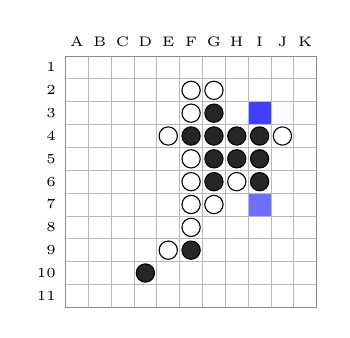
\begin{tikzpicture}[x=0.29cm, y=0.29cm]
\fill[blue!75] (8,-2) rectangle (9,-3);
\fill[blue!2] (9,-2) rectangle (10,-3);
\fill[blue!57] (8,-6) rectangle (9,-7);
\draw[gray!55, line width=.3pt, step=1] (0,0) grid (11,-11);
\draw[gray!90] (0,0) rectangle (11,-11);
\node[font=\tiny, anchor=south] at (0.5,0) {A};
\node[font=\tiny, anchor=south] at (1.5,0) {B};
\node[font=\tiny, anchor=south] at (2.5,0) {C};
\node[font=\tiny, anchor=south] at (3.5,0) {D};
\node[font=\tiny, anchor=south] at (4.5,0) {E};
\node[font=\tiny, anchor=south] at (5.5,0) {F};
\node[font=\tiny, anchor=south] at (6.5,0) {G};
\node[font=\tiny, anchor=south] at (7.5,0) {H};
\node[font=\tiny, anchor=south] at (8.5,0) {I};
\node[font=\tiny, anchor=south] at (9.5,0) {J};
\node[font=\tiny, anchor=south] at (10.5,0) {K};
\node[font=\tiny, anchor=east] at (0,-0.5) {1};
\node[font=\tiny, anchor=east] at (0,-1.5) {2};
\node[font=\tiny, anchor=east] at (0,-2.5) {3};
\node[font=\tiny, anchor=east] at (0,-3.5) {4};
\node[font=\tiny, anchor=east] at (0,-4.5) {5};
\node[font=\tiny, anchor=east] at (0,-5.5) {6};
\node[font=\tiny, anchor=east] at (0,-6.5) {7};
\node[font=\tiny, anchor=east] at (0,-7.5) {8};
\node[font=\tiny, anchor=east] at (0,-8.5) {9};
\node[font=\tiny, anchor=east] at (0,-9.5) {10};
\node[font=\tiny, anchor=east] at (0,-10.5) {11};
\draw[fill=white, line width=.4pt] (5.5,-1.5) circle (.40);
\draw[fill=white, line width=.4pt] (6.5,-1.5) circle (.40);
\draw[fill=white, line width=.4pt] (5.5,-2.5) circle (.40);
\draw[fill=black!85, line width=.4pt] (6.5,-2.5) circle (.40);
\draw[fill=white, line width=.4pt] (4.5,-3.5) circle (.40);
\draw[fill=black!85, line width=.4pt] (5.5,-3.5) circle (.40);
\draw[fill=black!85, line width=.4pt] (6.5,-3.5) circle (.40);
\draw[fill=black!85, line width=.4pt] (7.5,-3.5) circle (.40);
\draw[fill=black!85, line width=.4pt] (8.5,-3.5) circle (.40);
\draw[fill=white, line width=.4pt] (9.5,-3.5) circle (.40);
\draw[fill=white, line width=.4pt] (5.5,-4.5) circle (.40);
\draw[fill=black!85, line width=.4pt] (6.5,-4.5) circle (.40);
\draw[fill=black!85, line width=.4pt] (7.5,-4.5) circle (.40);
\draw[fill=black!85, line width=.4pt] (8.5,-4.5) circle (.40);
\draw[fill=white, line width=.4pt] (5.5,-5.5) circle (.40);
\draw[fill=black!85, line width=.4pt] (6.5,-5.5) circle (.40);
\draw[fill=white, line width=.4pt] (7.5,-5.5) circle (.40);
\draw[fill=black!85, line width=.4pt] (8.5,-5.5) circle (.40);
\draw[fill=white, line width=.4pt] (5.5,-6.5) circle (.40);
\draw[fill=white, line width=.4pt] (6.5,-6.5) circle (.40);
\draw[fill=white, line width=.4pt] (5.5,-7.5) circle (.40);
\draw[fill=white, line width=.4pt] (4.5,-8.5) circle (.40);
\draw[fill=black!85, line width=.4pt] (5.5,-8.5) circle (.40);
\draw[fill=black!85, line width=.4pt] (3.5,-9.5) circle (.40);
\end{tikzpicture}
    \caption{\footnotesize L8, 800: I3}
  \end{subfigure}\hfill
  \begin{subfigure}[t]{.32\linewidth}
    \centering
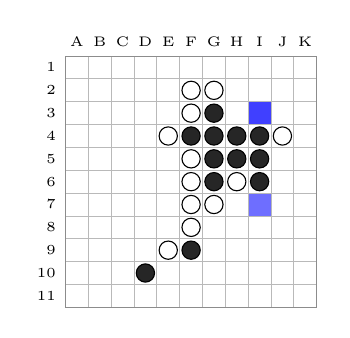
\begin{tikzpicture}[x=0.29cm, y=0.29cm]
\fill[blue!75] (8,-2) rectangle (9,-3);
\fill[blue!57] (8,-6) rectangle (9,-7);
\draw[gray!55, line width=.3pt, step=1] (0,0) grid (11,-11);
\draw[gray!90] (0,0) rectangle (11,-11);
\node[font=\tiny, anchor=south] at (0.5,0) {A};
\node[font=\tiny, anchor=south] at (1.5,0) {B};
\node[font=\tiny, anchor=south] at (2.5,0) {C};
\node[font=\tiny, anchor=south] at (3.5,0) {D};
\node[font=\tiny, anchor=south] at (4.5,0) {E};
\node[font=\tiny, anchor=south] at (5.5,0) {F};
\node[font=\tiny, anchor=south] at (6.5,0) {G};
\node[font=\tiny, anchor=south] at (7.5,0) {H};
\node[font=\tiny, anchor=south] at (8.5,0) {I};
\node[font=\tiny, anchor=south] at (9.5,0) {J};
\node[font=\tiny, anchor=south] at (10.5,0) {K};
\node[font=\tiny, anchor=east] at (0,-0.5) {1};
\node[font=\tiny, anchor=east] at (0,-1.5) {2};
\node[font=\tiny, anchor=east] at (0,-2.5) {3};
\node[font=\tiny, anchor=east] at (0,-3.5) {4};
\node[font=\tiny, anchor=east] at (0,-4.5) {5};
\node[font=\tiny, anchor=east] at (0,-5.5) {6};
\node[font=\tiny, anchor=east] at (0,-6.5) {7};
\node[font=\tiny, anchor=east] at (0,-7.5) {8};
\node[font=\tiny, anchor=east] at (0,-8.5) {9};
\node[font=\tiny, anchor=east] at (0,-9.5) {10};
\node[font=\tiny, anchor=east] at (0,-10.5) {11};
\draw[fill=white, line width=.4pt] (5.5,-1.5) circle (.40);
\draw[fill=white, line width=.4pt] (6.5,-1.5) circle (.40);
\draw[fill=white, line width=.4pt] (5.5,-2.5) circle (.40);
\draw[fill=black!85, line width=.4pt] (6.5,-2.5) circle (.40);
\draw[fill=white, line width=.4pt] (4.5,-3.5) circle (.40);
\draw[fill=black!85, line width=.4pt] (5.5,-3.5) circle (.40);
\draw[fill=black!85, line width=.4pt] (6.5,-3.5) circle (.40);
\draw[fill=black!85, line width=.4pt] (7.5,-3.5) circle (.40);
\draw[fill=black!85, line width=.4pt] (8.5,-3.5) circle (.40);
\draw[fill=white, line width=.4pt] (9.5,-3.5) circle (.40);
\draw[fill=white, line width=.4pt] (5.5,-4.5) circle (.40);
\draw[fill=black!85, line width=.4pt] (6.5,-4.5) circle (.40);
\draw[fill=black!85, line width=.4pt] (7.5,-4.5) circle (.40);
\draw[fill=black!85, line width=.4pt] (8.5,-4.5) circle (.40);
\draw[fill=white, line width=.4pt] (5.5,-5.5) circle (.40);
\draw[fill=black!85, line width=.4pt] (6.5,-5.5) circle (.40);
\draw[fill=white, line width=.4pt] (7.5,-5.5) circle (.40);
\draw[fill=black!85, line width=.4pt] (8.5,-5.5) circle (.40);
\draw[fill=white, line width=.4pt] (5.5,-6.5) circle (.40);
\draw[fill=white, line width=.4pt] (6.5,-6.5) circle (.40);
\draw[fill=white, line width=.4pt] (5.5,-7.5) circle (.40);
\draw[fill=white, line width=.4pt] (4.5,-8.5) circle (.40);
\draw[fill=black!85, line width=.4pt] (5.5,-8.5) circle (.40);
\draw[fill=black!85, line width=.4pt] (3.5,-9.5) circle (.40);
\end{tikzpicture}
    \caption{\footnotesize L8, 3.200: I3}
  \end{subfigure}\par\medskip
  \caption{Phân bố lượt thăm ở gốc tại thế C3-001 (X đi) khi tăng ngân sách. Đáp án: I2, K2, I3, J3, J5, K5. Chú thích con ghi nước được chọn.}
  \label{fig:cs-tham-c3-001}
\end{figure}

Ở thế C3-001 có 12 đáp án, mọi cấu hình trong bảng đều chọn đúng, nhưng theo cách khác nhau. L7 đặt $100\%$ lượt
thăm lên các đáp án ngay từ 50 mô phỏng, L8 đặt $90$--$99{,}8\%$, còn MCTS \texttt{light} chỉ đặt $20$--$60\%$ và rải phần
còn lại sang nước khác.
\begin{table}[H]
  \centering
  \footnotesize
  \caption{Tìm kiếm tại thế C5-001}
  \label{tab:cs-tk-nhiet-c5-001}
  \begin{tabular}{lrcrrl}
    \toprule
    Cấu hình & Mô phỏng & Chọn & Thăm đáp án (\%) & Q & Biến chính \\
    \midrule
    L4 light & 100 & G9 & 6,0 & 1,00 & G9 F9 \\
    L4 light & 800 & F9 & 29,1 & 0,62 & F9 G2 K4 \\
    L4 light & 6.400 & C8 & 18,6 & -0,05 & C8 E4 E3 \\
    L7 & 50 & C8 & 90,0 & 0,05 & C8 E4 E3 D8 D9 \\
    L7 & 800 & C8 & 89,1 & -0,05 & C8 D8 D9 E4 E3 \\
    L7 & 3.200 & C8 & 96,8 & -0,37 & C8 D8 D9 E4 E3 \\
    L8 & 50 & C8 & 22,0 & -0,41 & C8 D8 D9 G6 \\
    L8 & 800 & C8 & 85,9 & -0,85 & C8 D8 D9 E4 E3 \\
    L8 & 3.200 & C8 & 96,1 & -0,75 & C8 D8 D5 C7 B8 \\
    \bottomrule
  \end{tabular}
\end{table}

\begin{figure}[H]
  \centering
  \begin{subfigure}[t]{.32\linewidth}
    \centering
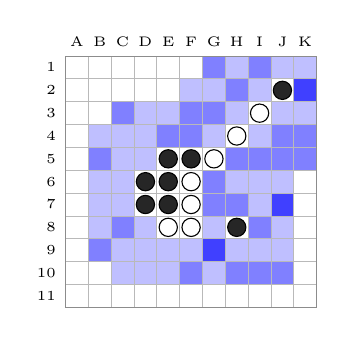
\begin{tikzpicture}[x=0.29cm, y=0.29cm]
\fill[blue!25] (7,-2) rectangle (8,-3);
\fill[blue!75] (6,-8) rectangle (7,-9);
\fill[blue!25] (3,-2) rectangle (4,-3);
\fill[blue!50] (7,-9) rectangle (8,-10);
\fill[blue!50] (6,-2) rectangle (7,-3);
\fill[blue!25] (2,-4) rectangle (3,-5);
\fill[blue!50] (10,-4) rectangle (11,-5);
\fill[blue!50] (5,-2) rectangle (6,-3);
\fill[blue!75] (9,-6) rectangle (10,-7);
\fill[blue!75] (10,-1) rectangle (11,-2);
\fill[blue!25] (2,-6) rectangle (3,-7);
\fill[blue!25] (3,-9) rectangle (4,-10);
\fill[blue!25] (9,-8) rectangle (10,-9);
\fill[blue!50] (7,-1) rectangle (8,-2);
\fill[blue!25] (7,0) rectangle (8,-1);
\fill[blue!50] (6,-5) rectangle (7,-6);
\fill[blue!25] (8,-6) rectangle (9,-7);
\fill[blue!50] (8,-7) rectangle (9,-8);
\fill[blue!25] (9,0) rectangle (10,-1);
\fill[blue!25] (6,-9) rectangle (7,-10);
\fill[blue!25] (6,-7) rectangle (7,-8);
\fill[blue!25] (4,-9) rectangle (5,-10);
\fill[blue!25] (9,-2) rectangle (10,-3);
\fill[blue!50] (1,-4) rectangle (2,-5);
\fill[blue!50] (1,-8) rectangle (2,-9);
\fill[blue!25] (8,-1) rectangle (9,-2);
\fill[blue!25] (2,-5) rectangle (3,-6);
\fill[blue!50] (2,-7) rectangle (3,-8);
\fill[blue!25] (1,-5) rectangle (2,-6);
\fill[blue!25] (6,-3) rectangle (7,-4);
\fill[blue!25] (10,-2) rectangle (11,-3);
\fill[blue!25] (7,-8) rectangle (8,-9);
\fill[blue!25] (3,-7) rectangle (4,-8);
\fill[blue!25] (5,-8) rectangle (6,-9);
\fill[blue!25] (4,-8) rectangle (5,-9);
\fill[blue!25] (7,-5) rectangle (8,-6);
\fill[blue!50] (9,-3) rectangle (10,-4);
\fill[blue!25] (2,-3) rectangle (3,-4);
\fill[blue!25] (4,-2) rectangle (5,-3);
\fill[blue!50] (8,0) rectangle (9,-1);
\fill[blue!50] (6,0) rectangle (7,-1);
\fill[blue!25] (8,-5) rectangle (9,-6);
\fill[blue!25] (6,-1) rectangle (7,-2);
\fill[blue!25] (3,-4) rectangle (4,-5);
\fill[blue!50] (10,-3) rectangle (11,-4);
\fill[blue!25] (2,-8) rectangle (3,-9);
\fill[blue!25] (1,-3) rectangle (2,-4);
\fill[blue!25] (3,-8) rectangle (4,-9);
\fill[blue!50] (7,-4) rectangle (8,-5);
\fill[blue!50] (9,-4) rectangle (10,-5);
\fill[blue!50] (5,-9) rectangle (6,-10);
\fill[blue!50] (5,-3) rectangle (6,-4);
\fill[blue!50] (8,-4) rectangle (9,-5);
\fill[blue!25] (1,-6) rectangle (2,-7);
\fill[blue!25] (8,-3) rectangle (9,-4);
\fill[blue!25] (3,-3) rectangle (4,-4);
\fill[blue!25] (10,0) rectangle (11,-1);
\fill[blue!50] (9,-9) rectangle (10,-10);
\fill[blue!25] (9,-5) rectangle (10,-6);
\fill[blue!25] (8,-8) rectangle (9,-9);
\fill[blue!25] (1,-7) rectangle (2,-8);
\fill[blue!25] (5,-1) rectangle (6,-2);
\fill[blue!50] (8,-9) rectangle (9,-10);
\fill[blue!50] (6,-6) rectangle (7,-7);
\fill[blue!50] (7,-6) rectangle (8,-7);
\fill[blue!50] (2,-2) rectangle (3,-3);
\fill[blue!25] (9,-7) rectangle (10,-8);
\fill[blue!25] (2,-9) rectangle (3,-10);
\fill[blue!50] (4,-3) rectangle (5,-4);
\draw[gray!55, line width=.3pt, step=1] (0,0) grid (11,-11);
\draw[gray!90] (0,0) rectangle (11,-11);
\node[font=\tiny, anchor=south] at (0.5,0) {A};
\node[font=\tiny, anchor=south] at (1.5,0) {B};
\node[font=\tiny, anchor=south] at (2.5,0) {C};
\node[font=\tiny, anchor=south] at (3.5,0) {D};
\node[font=\tiny, anchor=south] at (4.5,0) {E};
\node[font=\tiny, anchor=south] at (5.5,0) {F};
\node[font=\tiny, anchor=south] at (6.5,0) {G};
\node[font=\tiny, anchor=south] at (7.5,0) {H};
\node[font=\tiny, anchor=south] at (8.5,0) {I};
\node[font=\tiny, anchor=south] at (9.5,0) {J};
\node[font=\tiny, anchor=south] at (10.5,0) {K};
\node[font=\tiny, anchor=east] at (0,-0.5) {1};
\node[font=\tiny, anchor=east] at (0,-1.5) {2};
\node[font=\tiny, anchor=east] at (0,-2.5) {3};
\node[font=\tiny, anchor=east] at (0,-3.5) {4};
\node[font=\tiny, anchor=east] at (0,-4.5) {5};
\node[font=\tiny, anchor=east] at (0,-5.5) {6};
\node[font=\tiny, anchor=east] at (0,-6.5) {7};
\node[font=\tiny, anchor=east] at (0,-7.5) {8};
\node[font=\tiny, anchor=east] at (0,-8.5) {9};
\node[font=\tiny, anchor=east] at (0,-9.5) {10};
\node[font=\tiny, anchor=east] at (0,-10.5) {11};
\draw[fill=black!85, line width=.4pt] (9.5,-1.5) circle (.40);
\draw[fill=white, line width=.4pt] (8.5,-2.5) circle (.40);
\draw[fill=white, line width=.4pt] (7.5,-3.5) circle (.40);
\draw[fill=black!85, line width=.4pt] (4.5,-4.5) circle (.40);
\draw[fill=black!85, line width=.4pt] (5.5,-4.5) circle (.40);
\draw[fill=white, line width=.4pt] (6.5,-4.5) circle (.40);
\draw[fill=black!85, line width=.4pt] (3.5,-5.5) circle (.40);
\draw[fill=black!85, line width=.4pt] (4.5,-5.5) circle (.40);
\draw[fill=white, line width=.4pt] (5.5,-5.5) circle (.40);
\draw[fill=black!85, line width=.4pt] (3.5,-6.5) circle (.40);
\draw[fill=black!85, line width=.4pt] (4.5,-6.5) circle (.40);
\draw[fill=white, line width=.4pt] (5.5,-6.5) circle (.40);
\draw[fill=white, line width=.4pt] (4.5,-7.5) circle (.40);
\draw[fill=white, line width=.4pt] (5.5,-7.5) circle (.40);
\draw[fill=black!85, line width=.4pt] (7.5,-7.5) circle (.40);
\end{tikzpicture}
    \caption{\footnotesize L4 light, 100: G9}
  \end{subfigure}\hfill
  \begin{subfigure}[t]{.32\linewidth}
    \centering
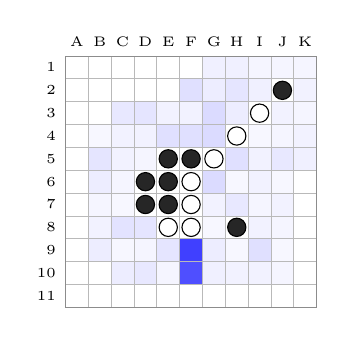
\begin{tikzpicture}[x=0.29cm, y=0.29cm]
\fill[blue!7] (7,-2) rectangle (8,-3);
\fill[blue!7] (6,-8) rectangle (7,-9);
\fill[blue!10] (3,-2) rectangle (4,-3);
\fill[blue!5] (7,-9) rectangle (8,-10);
\fill[blue!14] (6,-2) rectangle (7,-3);
\fill[blue!5] (2,-4) rectangle (3,-5);
\fill[blue!6] (10,-4) rectangle (11,-5);
\fill[blue!5] (5,-2) rectangle (6,-3);
\fill[blue!5] (9,-6) rectangle (10,-7);
\fill[blue!5] (10,-1) rectangle (11,-2);
\fill[blue!3] (2,-6) rectangle (3,-7);
\fill[blue!9] (3,-9) rectangle (4,-10);
\fill[blue!3] (9,-8) rectangle (10,-9);
\fill[blue!10] (7,-1) rectangle (8,-2);
\fill[blue!6] (7,0) rectangle (8,-1);
\fill[blue!14] (6,-5) rectangle (7,-6);
\fill[blue!4] (8,-6) rectangle (9,-7);
\fill[blue!5] (8,-7) rectangle (9,-8);
\fill[blue!4] (9,0) rectangle (10,-1);
\fill[blue!6] (6,-9) rectangle (7,-10);
\fill[blue!3] (6,-7) rectangle (7,-8);
\fill[blue!4] (4,-9) rectangle (5,-10);
\fill[blue!5] (9,-2) rectangle (10,-3);
\fill[blue!10] (1,-4) rectangle (2,-5);
\fill[blue!7] (1,-8) rectangle (2,-9);
\fill[blue!6] (8,-1) rectangle (9,-2);
\fill[blue!4] (2,-5) rectangle (3,-6);
\fill[blue!11] (2,-7) rectangle (3,-8);
\fill[blue!7] (1,-5) rectangle (2,-6);
\fill[blue!14] (6,-3) rectangle (7,-4);
\fill[blue!4] (10,-2) rectangle (11,-3);
\fill[blue!3] (7,-8) rectangle (8,-9);
\fill[blue!10] (3,-7) rectangle (4,-8);
\fill[blue!75] (5,-8) rectangle (6,-9);
\fill[blue!10] (4,-8) rectangle (5,-9);
\fill[blue!3] (7,-5) rectangle (8,-6);
\fill[blue!4] (9,-3) rectangle (10,-4);
\fill[blue!5] (2,-3) rectangle (3,-4);
\fill[blue!5] (4,-2) rectangle (5,-3);
\fill[blue!4] (8,0) rectangle (9,-1);
\fill[blue!6] (6,0) rectangle (7,-1);
\fill[blue!5] (8,-5) rectangle (9,-6);
\fill[blue!7] (6,-1) rectangle (7,-2);
\fill[blue!4] (3,-4) rectangle (4,-5);
\fill[blue!5] (10,-3) rectangle (11,-4);
\fill[blue!3] (2,-8) rectangle (3,-9);
\fill[blue!3] (1,-3) rectangle (2,-4);
\fill[blue!4] (3,-8) rectangle (4,-9);
\fill[blue!12] (7,-4) rectangle (8,-5);
\fill[blue!9] (9,-4) rectangle (10,-5);
\fill[blue!69] (5,-9) rectangle (6,-10);
\fill[blue!12] (5,-3) rectangle (6,-4);
\fill[blue!5] (8,-4) rectangle (9,-5);
\fill[blue!4] (1,-6) rectangle (2,-7);
\fill[blue!3] (8,-3) rectangle (9,-4);
\fill[blue!5] (3,-3) rectangle (4,-4);
\fill[blue!4] (10,0) rectangle (11,-1);
\fill[blue!4] (9,-9) rectangle (10,-10);
\fill[blue!3] (9,-5) rectangle (10,-6);
\fill[blue!12] (8,-8) rectangle (9,-9);
\fill[blue!5] (1,-7) rectangle (2,-8);
\fill[blue!12] (5,-1) rectangle (6,-2);
\fill[blue!5] (8,-9) rectangle (9,-10);
\fill[blue!5] (6,-6) rectangle (7,-7);
\fill[blue!9] (7,-6) rectangle (8,-7);
\fill[blue!9] (2,-2) rectangle (3,-3);
\fill[blue!4] (9,-7) rectangle (10,-8);
\fill[blue!7] (2,-9) rectangle (3,-10);
\fill[blue!12] (4,-3) rectangle (5,-4);
\draw[gray!55, line width=.3pt, step=1] (0,0) grid (11,-11);
\draw[gray!90] (0,0) rectangle (11,-11);
\node[font=\tiny, anchor=south] at (0.5,0) {A};
\node[font=\tiny, anchor=south] at (1.5,0) {B};
\node[font=\tiny, anchor=south] at (2.5,0) {C};
\node[font=\tiny, anchor=south] at (3.5,0) {D};
\node[font=\tiny, anchor=south] at (4.5,0) {E};
\node[font=\tiny, anchor=south] at (5.5,0) {F};
\node[font=\tiny, anchor=south] at (6.5,0) {G};
\node[font=\tiny, anchor=south] at (7.5,0) {H};
\node[font=\tiny, anchor=south] at (8.5,0) {I};
\node[font=\tiny, anchor=south] at (9.5,0) {J};
\node[font=\tiny, anchor=south] at (10.5,0) {K};
\node[font=\tiny, anchor=east] at (0,-0.5) {1};
\node[font=\tiny, anchor=east] at (0,-1.5) {2};
\node[font=\tiny, anchor=east] at (0,-2.5) {3};
\node[font=\tiny, anchor=east] at (0,-3.5) {4};
\node[font=\tiny, anchor=east] at (0,-4.5) {5};
\node[font=\tiny, anchor=east] at (0,-5.5) {6};
\node[font=\tiny, anchor=east] at (0,-6.5) {7};
\node[font=\tiny, anchor=east] at (0,-7.5) {8};
\node[font=\tiny, anchor=east] at (0,-8.5) {9};
\node[font=\tiny, anchor=east] at (0,-9.5) {10};
\node[font=\tiny, anchor=east] at (0,-10.5) {11};
\draw[fill=black!85, line width=.4pt] (9.5,-1.5) circle (.40);
\draw[fill=white, line width=.4pt] (8.5,-2.5) circle (.40);
\draw[fill=white, line width=.4pt] (7.5,-3.5) circle (.40);
\draw[fill=black!85, line width=.4pt] (4.5,-4.5) circle (.40);
\draw[fill=black!85, line width=.4pt] (5.5,-4.5) circle (.40);
\draw[fill=white, line width=.4pt] (6.5,-4.5) circle (.40);
\draw[fill=black!85, line width=.4pt] (3.5,-5.5) circle (.40);
\draw[fill=black!85, line width=.4pt] (4.5,-5.5) circle (.40);
\draw[fill=white, line width=.4pt] (5.5,-5.5) circle (.40);
\draw[fill=black!85, line width=.4pt] (3.5,-6.5) circle (.40);
\draw[fill=black!85, line width=.4pt] (4.5,-6.5) circle (.40);
\draw[fill=white, line width=.4pt] (5.5,-6.5) circle (.40);
\draw[fill=white, line width=.4pt] (4.5,-7.5) circle (.40);
\draw[fill=white, line width=.4pt] (5.5,-7.5) circle (.40);
\draw[fill=black!85, line width=.4pt] (7.5,-7.5) circle (.40);
\end{tikzpicture}
    \caption{\footnotesize L4 light, 800: F9}
  \end{subfigure}\hfill
  \begin{subfigure}[t]{.32\linewidth}
    \centering
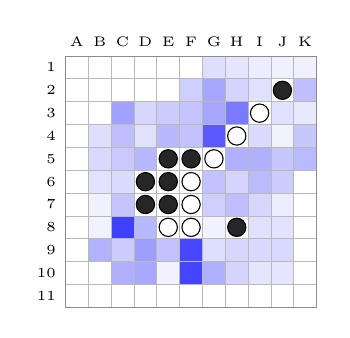
\begin{tikzpicture}[x=0.29cm, y=0.29cm]
\fill[blue!52] (7,-2) rectangle (8,-3);
\fill[blue!13] (6,-8) rectangle (7,-9);
\fill[blue!16] (3,-2) rectangle (4,-3);
\fill[blue!17] (7,-9) rectangle (8,-10);
\fill[blue!35] (6,-2) rectangle (7,-3);
\fill[blue!21] (2,-4) rectangle (3,-5);
\fill[blue!27] (10,-4) rectangle (11,-5);
\fill[blue!23] (5,-2) rectangle (6,-3);
\fill[blue!7] (9,-6) rectangle (10,-7);
\fill[blue!25] (10,-1) rectangle (11,-2);
\fill[blue!23] (2,-6) rectangle (3,-7);
\fill[blue!34] (3,-9) rectangle (4,-10);
\fill[blue!15] (9,-8) rectangle (10,-9);
\fill[blue!17] (7,-1) rectangle (8,-2);
\fill[blue!10] (7,0) rectangle (8,-1);
\fill[blue!24] (6,-5) rectangle (7,-6);
\fill[blue!16] (8,-6) rectangle (9,-7);
\fill[blue!12] (8,-7) rectangle (9,-8);
\fill[blue!6] (9,0) rectangle (10,-1);
\fill[blue!31] (6,-9) rectangle (7,-10);
\fill[blue!5] (6,-7) rectangle (7,-8);
\fill[blue!5] (4,-9) rectangle (5,-10);
\fill[blue!12] (9,-2) rectangle (10,-3);
\fill[blue!15] (1,-4) rectangle (2,-5);
\fill[blue!30] (1,-8) rectangle (2,-9);
\fill[blue!12] (8,-1) rectangle (9,-2);
\fill[blue!14] (2,-5) rectangle (3,-6);
\fill[blue!75] (2,-7) rectangle (3,-8);
\fill[blue!11] (1,-5) rectangle (2,-6);
\fill[blue!65] (6,-3) rectangle (7,-4);
\fill[blue!9] (10,-2) rectangle (11,-3);
\fill[blue!16] (7,-8) rectangle (8,-9);
\fill[blue!28] (3,-7) rectangle (4,-8);
\fill[blue!72] (5,-8) rectangle (6,-9);
\fill[blue!24] (4,-8) rectangle (5,-9);
\fill[blue!17] (7,-5) rectangle (8,-6);
\fill[blue!5] (9,-3) rectangle (10,-4);
\fill[blue!25] (2,-3) rectangle (3,-4);
\fill[blue!20] (4,-2) rectangle (5,-3);
\fill[blue!7] (8,0) rectangle (9,-1);
\fill[blue!13] (6,0) rectangle (7,-1);
\fill[blue!27] (8,-5) rectangle (9,-6);
\fill[blue!35] (6,-1) rectangle (7,-2);
\fill[blue!28] (3,-4) rectangle (4,-5);
\fill[blue!22] (10,-3) rectangle (11,-4);
\fill[blue!20] (2,-8) rectangle (3,-9);
\fill[blue!13] (1,-3) rectangle (2,-4);
\fill[blue!38] (3,-8) rectangle (4,-9);
\fill[blue!31] (7,-4) rectangle (8,-5);
\fill[blue!22] (9,-4) rectangle (10,-5);
\fill[blue!73] (5,-9) rectangle (6,-10);
\fill[blue!24] (5,-3) rectangle (6,-4);
\fill[blue!31] (8,-4) rectangle (9,-5);
\fill[blue!6] (1,-6) rectangle (2,-7);
\fill[blue!14] (8,-3) rectangle (9,-4);
\fill[blue!12] (3,-3) rectangle (4,-4);
\fill[blue!6] (10,0) rectangle (11,-1);
\fill[blue!10] (9,-9) rectangle (10,-10);
\fill[blue!20] (9,-5) rectangle (10,-6);
\fill[blue!15] (8,-8) rectangle (9,-9);
\fill[blue!5] (1,-7) rectangle (2,-8);
\fill[blue!19] (5,-1) rectangle (6,-2);
\fill[blue!10] (8,-9) rectangle (9,-10);
\fill[blue!19] (6,-6) rectangle (7,-7);
\fill[blue!25] (7,-6) rectangle (8,-7);
\fill[blue!37] (2,-2) rectangle (3,-3);
\fill[blue!11] (9,-7) rectangle (10,-8);
\fill[blue!31] (2,-9) rectangle (3,-10);
\fill[blue!28] (4,-3) rectangle (5,-4);
\draw[gray!55, line width=.3pt, step=1] (0,0) grid (11,-11);
\draw[gray!90] (0,0) rectangle (11,-11);
\node[font=\tiny, anchor=south] at (0.5,0) {A};
\node[font=\tiny, anchor=south] at (1.5,0) {B};
\node[font=\tiny, anchor=south] at (2.5,0) {C};
\node[font=\tiny, anchor=south] at (3.5,0) {D};
\node[font=\tiny, anchor=south] at (4.5,0) {E};
\node[font=\tiny, anchor=south] at (5.5,0) {F};
\node[font=\tiny, anchor=south] at (6.5,0) {G};
\node[font=\tiny, anchor=south] at (7.5,0) {H};
\node[font=\tiny, anchor=south] at (8.5,0) {I};
\node[font=\tiny, anchor=south] at (9.5,0) {J};
\node[font=\tiny, anchor=south] at (10.5,0) {K};
\node[font=\tiny, anchor=east] at (0,-0.5) {1};
\node[font=\tiny, anchor=east] at (0,-1.5) {2};
\node[font=\tiny, anchor=east] at (0,-2.5) {3};
\node[font=\tiny, anchor=east] at (0,-3.5) {4};
\node[font=\tiny, anchor=east] at (0,-4.5) {5};
\node[font=\tiny, anchor=east] at (0,-5.5) {6};
\node[font=\tiny, anchor=east] at (0,-6.5) {7};
\node[font=\tiny, anchor=east] at (0,-7.5) {8};
\node[font=\tiny, anchor=east] at (0,-8.5) {9};
\node[font=\tiny, anchor=east] at (0,-9.5) {10};
\node[font=\tiny, anchor=east] at (0,-10.5) {11};
\draw[fill=black!85, line width=.4pt] (9.5,-1.5) circle (.40);
\draw[fill=white, line width=.4pt] (8.5,-2.5) circle (.40);
\draw[fill=white, line width=.4pt] (7.5,-3.5) circle (.40);
\draw[fill=black!85, line width=.4pt] (4.5,-4.5) circle (.40);
\draw[fill=black!85, line width=.4pt] (5.5,-4.5) circle (.40);
\draw[fill=white, line width=.4pt] (6.5,-4.5) circle (.40);
\draw[fill=black!85, line width=.4pt] (3.5,-5.5) circle (.40);
\draw[fill=black!85, line width=.4pt] (4.5,-5.5) circle (.40);
\draw[fill=white, line width=.4pt] (5.5,-5.5) circle (.40);
\draw[fill=black!85, line width=.4pt] (3.5,-6.5) circle (.40);
\draw[fill=black!85, line width=.4pt] (4.5,-6.5) circle (.40);
\draw[fill=white, line width=.4pt] (5.5,-6.5) circle (.40);
\draw[fill=white, line width=.4pt] (4.5,-7.5) circle (.40);
\draw[fill=white, line width=.4pt] (5.5,-7.5) circle (.40);
\draw[fill=black!85, line width=.4pt] (7.5,-7.5) circle (.40);
\end{tikzpicture}
    \caption{\footnotesize L4 light, 6.400: C8}
  \end{subfigure}\par\medskip
  \begin{subfigure}[t]{.32\linewidth}
    \centering
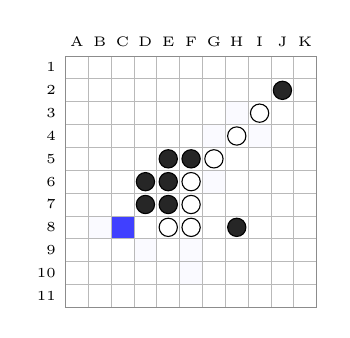
\begin{tikzpicture}[x=0.29cm, y=0.29cm]
\fill[blue!2] (7,-2) rectangle (8,-3);
\fill[blue!2] (6,-3) rectangle (7,-4);
\fill[blue!2] (8,-3) rectangle (9,-4);
\fill[blue!2] (6,-5) rectangle (7,-6);
\fill[blue!2] (1,-7) rectangle (2,-8);
\fill[blue!75] (2,-7) rectangle (3,-8);
\fill[blue!2] (3,-8) rectangle (4,-9);
\fill[blue!2] (5,-8) rectangle (6,-9);
\fill[blue!2] (5,-9) rectangle (6,-10);
\draw[gray!55, line width=.3pt, step=1] (0,0) grid (11,-11);
\draw[gray!90] (0,0) rectangle (11,-11);
\node[font=\tiny, anchor=south] at (0.5,0) {A};
\node[font=\tiny, anchor=south] at (1.5,0) {B};
\node[font=\tiny, anchor=south] at (2.5,0) {C};
\node[font=\tiny, anchor=south] at (3.5,0) {D};
\node[font=\tiny, anchor=south] at (4.5,0) {E};
\node[font=\tiny, anchor=south] at (5.5,0) {F};
\node[font=\tiny, anchor=south] at (6.5,0) {G};
\node[font=\tiny, anchor=south] at (7.5,0) {H};
\node[font=\tiny, anchor=south] at (8.5,0) {I};
\node[font=\tiny, anchor=south] at (9.5,0) {J};
\node[font=\tiny, anchor=south] at (10.5,0) {K};
\node[font=\tiny, anchor=east] at (0,-0.5) {1};
\node[font=\tiny, anchor=east] at (0,-1.5) {2};
\node[font=\tiny, anchor=east] at (0,-2.5) {3};
\node[font=\tiny, anchor=east] at (0,-3.5) {4};
\node[font=\tiny, anchor=east] at (0,-4.5) {5};
\node[font=\tiny, anchor=east] at (0,-5.5) {6};
\node[font=\tiny, anchor=east] at (0,-6.5) {7};
\node[font=\tiny, anchor=east] at (0,-7.5) {8};
\node[font=\tiny, anchor=east] at (0,-8.5) {9};
\node[font=\tiny, anchor=east] at (0,-9.5) {10};
\node[font=\tiny, anchor=east] at (0,-10.5) {11};
\draw[fill=black!85, line width=.4pt] (9.5,-1.5) circle (.40);
\draw[fill=white, line width=.4pt] (8.5,-2.5) circle (.40);
\draw[fill=white, line width=.4pt] (7.5,-3.5) circle (.40);
\draw[fill=black!85, line width=.4pt] (4.5,-4.5) circle (.40);
\draw[fill=black!85, line width=.4pt] (5.5,-4.5) circle (.40);
\draw[fill=white, line width=.4pt] (6.5,-4.5) circle (.40);
\draw[fill=black!85, line width=.4pt] (3.5,-5.5) circle (.40);
\draw[fill=black!85, line width=.4pt] (4.5,-5.5) circle (.40);
\draw[fill=white, line width=.4pt] (5.5,-5.5) circle (.40);
\draw[fill=black!85, line width=.4pt] (3.5,-6.5) circle (.40);
\draw[fill=black!85, line width=.4pt] (4.5,-6.5) circle (.40);
\draw[fill=white, line width=.4pt] (5.5,-6.5) circle (.40);
\draw[fill=white, line width=.4pt] (4.5,-7.5) circle (.40);
\draw[fill=white, line width=.4pt] (5.5,-7.5) circle (.40);
\draw[fill=black!85, line width=.4pt] (7.5,-7.5) circle (.40);
\end{tikzpicture}
    \caption{\footnotesize L7, 50: C8}
  \end{subfigure}\hfill
  \begin{subfigure}[t]{.32\linewidth}
    \centering
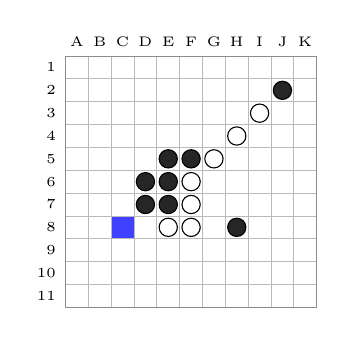
\begin{tikzpicture}[x=0.29cm, y=0.29cm]
\fill[blue!75] (2,-7) rectangle (3,-8);
\draw[gray!55, line width=.3pt, step=1] (0,0) grid (11,-11);
\draw[gray!90] (0,0) rectangle (11,-11);
\node[font=\tiny, anchor=south] at (0.5,0) {A};
\node[font=\tiny, anchor=south] at (1.5,0) {B};
\node[font=\tiny, anchor=south] at (2.5,0) {C};
\node[font=\tiny, anchor=south] at (3.5,0) {D};
\node[font=\tiny, anchor=south] at (4.5,0) {E};
\node[font=\tiny, anchor=south] at (5.5,0) {F};
\node[font=\tiny, anchor=south] at (6.5,0) {G};
\node[font=\tiny, anchor=south] at (7.5,0) {H};
\node[font=\tiny, anchor=south] at (8.5,0) {I};
\node[font=\tiny, anchor=south] at (9.5,0) {J};
\node[font=\tiny, anchor=south] at (10.5,0) {K};
\node[font=\tiny, anchor=east] at (0,-0.5) {1};
\node[font=\tiny, anchor=east] at (0,-1.5) {2};
\node[font=\tiny, anchor=east] at (0,-2.5) {3};
\node[font=\tiny, anchor=east] at (0,-3.5) {4};
\node[font=\tiny, anchor=east] at (0,-4.5) {5};
\node[font=\tiny, anchor=east] at (0,-5.5) {6};
\node[font=\tiny, anchor=east] at (0,-6.5) {7};
\node[font=\tiny, anchor=east] at (0,-7.5) {8};
\node[font=\tiny, anchor=east] at (0,-8.5) {9};
\node[font=\tiny, anchor=east] at (0,-9.5) {10};
\node[font=\tiny, anchor=east] at (0,-10.5) {11};
\draw[fill=black!85, line width=.4pt] (9.5,-1.5) circle (.40);
\draw[fill=white, line width=.4pt] (8.5,-2.5) circle (.40);
\draw[fill=white, line width=.4pt] (7.5,-3.5) circle (.40);
\draw[fill=black!85, line width=.4pt] (4.5,-4.5) circle (.40);
\draw[fill=black!85, line width=.4pt] (5.5,-4.5) circle (.40);
\draw[fill=white, line width=.4pt] (6.5,-4.5) circle (.40);
\draw[fill=black!85, line width=.4pt] (3.5,-5.5) circle (.40);
\draw[fill=black!85, line width=.4pt] (4.5,-5.5) circle (.40);
\draw[fill=white, line width=.4pt] (5.5,-5.5) circle (.40);
\draw[fill=black!85, line width=.4pt] (3.5,-6.5) circle (.40);
\draw[fill=black!85, line width=.4pt] (4.5,-6.5) circle (.40);
\draw[fill=white, line width=.4pt] (5.5,-6.5) circle (.40);
\draw[fill=white, line width=.4pt] (4.5,-7.5) circle (.40);
\draw[fill=white, line width=.4pt] (5.5,-7.5) circle (.40);
\draw[fill=black!85, line width=.4pt] (7.5,-7.5) circle (.40);
\end{tikzpicture}
    \caption{\footnotesize L7, 800: C8}
  \end{subfigure}\hfill
  \begin{subfigure}[t]{.32\linewidth}
    \centering
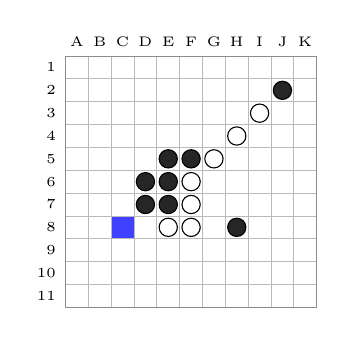
\begin{tikzpicture}[x=0.29cm, y=0.29cm]
\fill[blue!75] (2,-7) rectangle (3,-8);
\draw[gray!55, line width=.3pt, step=1] (0,0) grid (11,-11);
\draw[gray!90] (0,0) rectangle (11,-11);
\node[font=\tiny, anchor=south] at (0.5,0) {A};
\node[font=\tiny, anchor=south] at (1.5,0) {B};
\node[font=\tiny, anchor=south] at (2.5,0) {C};
\node[font=\tiny, anchor=south] at (3.5,0) {D};
\node[font=\tiny, anchor=south] at (4.5,0) {E};
\node[font=\tiny, anchor=south] at (5.5,0) {F};
\node[font=\tiny, anchor=south] at (6.5,0) {G};
\node[font=\tiny, anchor=south] at (7.5,0) {H};
\node[font=\tiny, anchor=south] at (8.5,0) {I};
\node[font=\tiny, anchor=south] at (9.5,0) {J};
\node[font=\tiny, anchor=south] at (10.5,0) {K};
\node[font=\tiny, anchor=east] at (0,-0.5) {1};
\node[font=\tiny, anchor=east] at (0,-1.5) {2};
\node[font=\tiny, anchor=east] at (0,-2.5) {3};
\node[font=\tiny, anchor=east] at (0,-3.5) {4};
\node[font=\tiny, anchor=east] at (0,-4.5) {5};
\node[font=\tiny, anchor=east] at (0,-5.5) {6};
\node[font=\tiny, anchor=east] at (0,-6.5) {7};
\node[font=\tiny, anchor=east] at (0,-7.5) {8};
\node[font=\tiny, anchor=east] at (0,-8.5) {9};
\node[font=\tiny, anchor=east] at (0,-9.5) {10};
\node[font=\tiny, anchor=east] at (0,-10.5) {11};
\draw[fill=black!85, line width=.4pt] (9.5,-1.5) circle (.40);
\draw[fill=white, line width=.4pt] (8.5,-2.5) circle (.40);
\draw[fill=white, line width=.4pt] (7.5,-3.5) circle (.40);
\draw[fill=black!85, line width=.4pt] (4.5,-4.5) circle (.40);
\draw[fill=black!85, line width=.4pt] (5.5,-4.5) circle (.40);
\draw[fill=white, line width=.4pt] (6.5,-4.5) circle (.40);
\draw[fill=black!85, line width=.4pt] (3.5,-5.5) circle (.40);
\draw[fill=black!85, line width=.4pt] (4.5,-5.5) circle (.40);
\draw[fill=white, line width=.4pt] (5.5,-5.5) circle (.40);
\draw[fill=black!85, line width=.4pt] (3.5,-6.5) circle (.40);
\draw[fill=black!85, line width=.4pt] (4.5,-6.5) circle (.40);
\draw[fill=white, line width=.4pt] (5.5,-6.5) circle (.40);
\draw[fill=white, line width=.4pt] (4.5,-7.5) circle (.40);
\draw[fill=white, line width=.4pt] (5.5,-7.5) circle (.40);
\draw[fill=black!85, line width=.4pt] (7.5,-7.5) circle (.40);
\end{tikzpicture}
    \caption{\footnotesize L7, 3.200: C8}
  \end{subfigure}\par\medskip
  \begin{subfigure}[t]{.32\linewidth}
    \centering
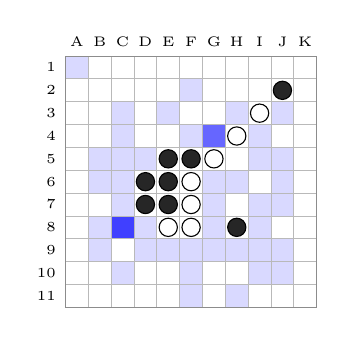
\begin{tikzpicture}[x=0.29cm, y=0.29cm]
\fill[blue!15] (0,0) rectangle (1,-1);
\fill[blue!15] (5,-1) rectangle (6,-2);
\fill[blue!15] (2,-2) rectangle (3,-3);
\fill[blue!15] (4,-2) rectangle (5,-3);
\fill[blue!15] (7,-2) rectangle (8,-3);
\fill[blue!15] (9,-2) rectangle (10,-3);
\fill[blue!15] (2,-3) rectangle (3,-4);
\fill[blue!15] (5,-3) rectangle (6,-4);
\fill[blue!60] (6,-3) rectangle (7,-4);
\fill[blue!15] (8,-3) rectangle (9,-4);
\fill[blue!15] (1,-4) rectangle (2,-5);
\fill[blue!15] (2,-4) rectangle (3,-5);
\fill[blue!15] (3,-4) rectangle (4,-5);
\fill[blue!15] (8,-4) rectangle (9,-5);
\fill[blue!15] (9,-4) rectangle (10,-5);
\fill[blue!15] (1,-5) rectangle (2,-6);
\fill[blue!15] (2,-5) rectangle (3,-6);
\fill[blue!15] (6,-5) rectangle (7,-6);
\fill[blue!15] (7,-5) rectangle (8,-6);
\fill[blue!15] (9,-5) rectangle (10,-6);
\fill[blue!15] (2,-6) rectangle (3,-7);
\fill[blue!15] (6,-6) rectangle (7,-7);
\fill[blue!15] (8,-6) rectangle (9,-7);
\fill[blue!15] (9,-6) rectangle (10,-7);
\fill[blue!15] (1,-7) rectangle (2,-8);
\fill[blue!75] (2,-7) rectangle (3,-8);
\fill[blue!15] (3,-7) rectangle (4,-8);
\fill[blue!15] (6,-7) rectangle (7,-8);
\fill[blue!15] (8,-7) rectangle (9,-8);
\fill[blue!15] (1,-8) rectangle (2,-9);
\fill[blue!15] (3,-8) rectangle (4,-9);
\fill[blue!15] (4,-8) rectangle (5,-9);
\fill[blue!15] (5,-8) rectangle (6,-9);
\fill[blue!15] (6,-8) rectangle (7,-9);
\fill[blue!15] (7,-8) rectangle (8,-9);
\fill[blue!15] (8,-8) rectangle (9,-9);
\fill[blue!15] (9,-8) rectangle (10,-9);
\fill[blue!15] (2,-9) rectangle (3,-10);
\fill[blue!15] (5,-9) rectangle (6,-10);
\fill[blue!15] (8,-9) rectangle (9,-10);
\fill[blue!15] (9,-9) rectangle (10,-10);
\fill[blue!15] (5,-10) rectangle (6,-11);
\fill[blue!15] (7,-10) rectangle (8,-11);
\draw[gray!55, line width=.3pt, step=1] (0,0) grid (11,-11);
\draw[gray!90] (0,0) rectangle (11,-11);
\node[font=\tiny, anchor=south] at (0.5,0) {A};
\node[font=\tiny, anchor=south] at (1.5,0) {B};
\node[font=\tiny, anchor=south] at (2.5,0) {C};
\node[font=\tiny, anchor=south] at (3.5,0) {D};
\node[font=\tiny, anchor=south] at (4.5,0) {E};
\node[font=\tiny, anchor=south] at (5.5,0) {F};
\node[font=\tiny, anchor=south] at (6.5,0) {G};
\node[font=\tiny, anchor=south] at (7.5,0) {H};
\node[font=\tiny, anchor=south] at (8.5,0) {I};
\node[font=\tiny, anchor=south] at (9.5,0) {J};
\node[font=\tiny, anchor=south] at (10.5,0) {K};
\node[font=\tiny, anchor=east] at (0,-0.5) {1};
\node[font=\tiny, anchor=east] at (0,-1.5) {2};
\node[font=\tiny, anchor=east] at (0,-2.5) {3};
\node[font=\tiny, anchor=east] at (0,-3.5) {4};
\node[font=\tiny, anchor=east] at (0,-4.5) {5};
\node[font=\tiny, anchor=east] at (0,-5.5) {6};
\node[font=\tiny, anchor=east] at (0,-6.5) {7};
\node[font=\tiny, anchor=east] at (0,-7.5) {8};
\node[font=\tiny, anchor=east] at (0,-8.5) {9};
\node[font=\tiny, anchor=east] at (0,-9.5) {10};
\node[font=\tiny, anchor=east] at (0,-10.5) {11};
\draw[fill=black!85, line width=.4pt] (9.5,-1.5) circle (.40);
\draw[fill=white, line width=.4pt] (8.5,-2.5) circle (.40);
\draw[fill=white, line width=.4pt] (7.5,-3.5) circle (.40);
\draw[fill=black!85, line width=.4pt] (4.5,-4.5) circle (.40);
\draw[fill=black!85, line width=.4pt] (5.5,-4.5) circle (.40);
\draw[fill=white, line width=.4pt] (6.5,-4.5) circle (.40);
\draw[fill=black!85, line width=.4pt] (3.5,-5.5) circle (.40);
\draw[fill=black!85, line width=.4pt] (4.5,-5.5) circle (.40);
\draw[fill=white, line width=.4pt] (5.5,-5.5) circle (.40);
\draw[fill=black!85, line width=.4pt] (3.5,-6.5) circle (.40);
\draw[fill=black!85, line width=.4pt] (4.5,-6.5) circle (.40);
\draw[fill=white, line width=.4pt] (5.5,-6.5) circle (.40);
\draw[fill=white, line width=.4pt] (4.5,-7.5) circle (.40);
\draw[fill=white, line width=.4pt] (5.5,-7.5) circle (.40);
\draw[fill=black!85, line width=.4pt] (7.5,-7.5) circle (.40);
\end{tikzpicture}
    \caption{\footnotesize L8, 50: C8}
  \end{subfigure}\hfill
  \begin{subfigure}[t]{.32\linewidth}
    \centering
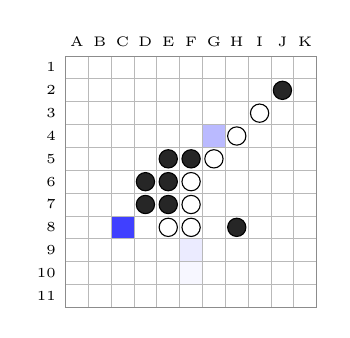
\begin{tikzpicture}[x=0.29cm, y=0.29cm]
\fill[blue!27] (6,-3) rectangle (7,-4);
\fill[blue!75] (2,-7) rectangle (3,-8);
\fill[blue!8] (5,-8) rectangle (6,-9);
\fill[blue!3] (5,-9) rectangle (6,-10);
\draw[gray!55, line width=.3pt, step=1] (0,0) grid (11,-11);
\draw[gray!90] (0,0) rectangle (11,-11);
\node[font=\tiny, anchor=south] at (0.5,0) {A};
\node[font=\tiny, anchor=south] at (1.5,0) {B};
\node[font=\tiny, anchor=south] at (2.5,0) {C};
\node[font=\tiny, anchor=south] at (3.5,0) {D};
\node[font=\tiny, anchor=south] at (4.5,0) {E};
\node[font=\tiny, anchor=south] at (5.5,0) {F};
\node[font=\tiny, anchor=south] at (6.5,0) {G};
\node[font=\tiny, anchor=south] at (7.5,0) {H};
\node[font=\tiny, anchor=south] at (8.5,0) {I};
\node[font=\tiny, anchor=south] at (9.5,0) {J};
\node[font=\tiny, anchor=south] at (10.5,0) {K};
\node[font=\tiny, anchor=east] at (0,-0.5) {1};
\node[font=\tiny, anchor=east] at (0,-1.5) {2};
\node[font=\tiny, anchor=east] at (0,-2.5) {3};
\node[font=\tiny, anchor=east] at (0,-3.5) {4};
\node[font=\tiny, anchor=east] at (0,-4.5) {5};
\node[font=\tiny, anchor=east] at (0,-5.5) {6};
\node[font=\tiny, anchor=east] at (0,-6.5) {7};
\node[font=\tiny, anchor=east] at (0,-7.5) {8};
\node[font=\tiny, anchor=east] at (0,-8.5) {9};
\node[font=\tiny, anchor=east] at (0,-9.5) {10};
\node[font=\tiny, anchor=east] at (0,-10.5) {11};
\draw[fill=black!85, line width=.4pt] (9.5,-1.5) circle (.40);
\draw[fill=white, line width=.4pt] (8.5,-2.5) circle (.40);
\draw[fill=white, line width=.4pt] (7.5,-3.5) circle (.40);
\draw[fill=black!85, line width=.4pt] (4.5,-4.5) circle (.40);
\draw[fill=black!85, line width=.4pt] (5.5,-4.5) circle (.40);
\draw[fill=white, line width=.4pt] (6.5,-4.5) circle (.40);
\draw[fill=black!85, line width=.4pt] (3.5,-5.5) circle (.40);
\draw[fill=black!85, line width=.4pt] (4.5,-5.5) circle (.40);
\draw[fill=white, line width=.4pt] (5.5,-5.5) circle (.40);
\draw[fill=black!85, line width=.4pt] (3.5,-6.5) circle (.40);
\draw[fill=black!85, line width=.4pt] (4.5,-6.5) circle (.40);
\draw[fill=white, line width=.4pt] (5.5,-6.5) circle (.40);
\draw[fill=white, line width=.4pt] (4.5,-7.5) circle (.40);
\draw[fill=white, line width=.4pt] (5.5,-7.5) circle (.40);
\draw[fill=black!85, line width=.4pt] (7.5,-7.5) circle (.40);
\end{tikzpicture}
    \caption{\footnotesize L8, 800: C8}
  \end{subfigure}\hfill
  \begin{subfigure}[t]{.32\linewidth}
    \centering
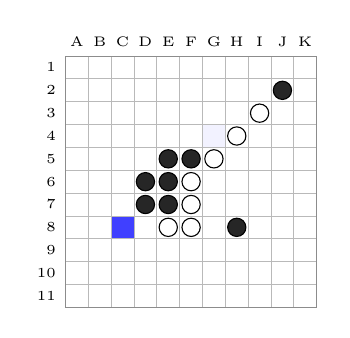
\begin{tikzpicture}[x=0.29cm, y=0.29cm]
\fill[blue!5] (6,-3) rectangle (7,-4);
\fill[blue!75] (2,-7) rectangle (3,-8);
\draw[gray!55, line width=.3pt, step=1] (0,0) grid (11,-11);
\draw[gray!90] (0,0) rectangle (11,-11);
\node[font=\tiny, anchor=south] at (0.5,0) {A};
\node[font=\tiny, anchor=south] at (1.5,0) {B};
\node[font=\tiny, anchor=south] at (2.5,0) {C};
\node[font=\tiny, anchor=south] at (3.5,0) {D};
\node[font=\tiny, anchor=south] at (4.5,0) {E};
\node[font=\tiny, anchor=south] at (5.5,0) {F};
\node[font=\tiny, anchor=south] at (6.5,0) {G};
\node[font=\tiny, anchor=south] at (7.5,0) {H};
\node[font=\tiny, anchor=south] at (8.5,0) {I};
\node[font=\tiny, anchor=south] at (9.5,0) {J};
\node[font=\tiny, anchor=south] at (10.5,0) {K};
\node[font=\tiny, anchor=east] at (0,-0.5) {1};
\node[font=\tiny, anchor=east] at (0,-1.5) {2};
\node[font=\tiny, anchor=east] at (0,-2.5) {3};
\node[font=\tiny, anchor=east] at (0,-3.5) {4};
\node[font=\tiny, anchor=east] at (0,-4.5) {5};
\node[font=\tiny, anchor=east] at (0,-5.5) {6};
\node[font=\tiny, anchor=east] at (0,-6.5) {7};
\node[font=\tiny, anchor=east] at (0,-7.5) {8};
\node[font=\tiny, anchor=east] at (0,-8.5) {9};
\node[font=\tiny, anchor=east] at (0,-9.5) {10};
\node[font=\tiny, anchor=east] at (0,-10.5) {11};
\draw[fill=black!85, line width=.4pt] (9.5,-1.5) circle (.40);
\draw[fill=white, line width=.4pt] (8.5,-2.5) circle (.40);
\draw[fill=white, line width=.4pt] (7.5,-3.5) circle (.40);
\draw[fill=black!85, line width=.4pt] (4.5,-4.5) circle (.40);
\draw[fill=black!85, line width=.4pt] (5.5,-4.5) circle (.40);
\draw[fill=white, line width=.4pt] (6.5,-4.5) circle (.40);
\draw[fill=black!85, line width=.4pt] (3.5,-5.5) circle (.40);
\draw[fill=black!85, line width=.4pt] (4.5,-5.5) circle (.40);
\draw[fill=white, line width=.4pt] (5.5,-5.5) circle (.40);
\draw[fill=black!85, line width=.4pt] (3.5,-6.5) circle (.40);
\draw[fill=black!85, line width=.4pt] (4.5,-6.5) circle (.40);
\draw[fill=white, line width=.4pt] (5.5,-6.5) circle (.40);
\draw[fill=white, line width=.4pt] (4.5,-7.5) circle (.40);
\draw[fill=white, line width=.4pt] (5.5,-7.5) circle (.40);
\draw[fill=black!85, line width=.4pt] (7.5,-7.5) circle (.40);
\end{tikzpicture}
    \caption{\footnotesize L8, 3.200: C8}
  \end{subfigure}\par\medskip
  \caption{Phân bố lượt thăm ở gốc tại thế C5-001 (O đi) khi tăng ngân sách. Đáp án: G4, C8, F9, F10. Chú thích con ghi nước được chọn.}
  \label{fig:cs-tham-c5-001}
\end{figure}

Ở thế phòng thủ C5-001 (đáp án G4, C8, F9, F10), L7 và L8 chọn C8 ở mọi mức. L8 ở 50 mô phỏng mới đặt $22\%$ lượt thăm
lên đáp án dù đã chọn C8, rồi tăng lên $96\%$ ở 3\,200. Giá trị $Q$ của nước chọn giảm khi tìm sâu hơn (L8: từ
$-0{,}41$ xuống khoảng $-0{,}8$): tìm kiếm phát hiện thế xấu hơn mức mạng đánh giá ban đầu. MCTS \texttt{light} chọn sai
ở 100 mô phỏng và đúng ở các mức lớn hơn.

\section{Tổng hợp phần phân tích chuyên sâu}
\begin{table}[H]
  \centering\small
  \caption{Câu hỏi, bằng chứng và mức chắc chắn của phần phân tích chuyên sâu}
  \label{tab:cs-tong-hop}
  \begin{tabular}{p{4.6cm}p{6.4cm}p{3cm}}
    \toprule
    Phát hiện & Bằng chứng & Mức chắc chắn\\
    \midrule
    Nhãn huấn luyện có hai lỗi & Đếm trên toàn tập, tái hiện bằng L3, đo trên bốn mạng & Cao\\
    Sửa lỗi nhãn làm mạnh hơn & Chưa huấn luyện lại & Chưa biết\\
    Rollout \texttt{light} bỏ chặn do mở rộng cây & 100 thế, đo trực tiếp rollout và cây & Cao trên loại thế đó\\
    P4 trước P5 làm mất chuỗi tứ & Bỏ luật trên 100 thế C4 & Cao trên bộ thế; chưa đấu\\
    Gốc Alpha-Beta bỏ phí thứ tự & 50 thế, hai độ sâu & Cao; lợi ích nhỏ\\
    L8 mạnh lên theo mô phỏng & 100 ván mỗi mức, một đối thủ & Trung bình\\
    $c_{puct}$ tối ưu gần 1,0 & 100 ván mỗi mức, khoảng chồng nhau & Thấp\\
    \bottomrule
  \end{tabular}
\end{table}
